\chapter{Области на Скот}\index{област на Скот}

\marginpar{\cite[Глава 5]{models-of-computation}}

В тази глава ще разгледаме понятията, които са ни нужни за дефинирането на понятието денотационна семантика на една програма.

\section{Частични наредби}
\index{частична наредба}

Бинарната релация $\sqsubseteq$ върху множеството $A$ се нарича {\bf частична наредба}, ако тя е:
\marginpar{На англ. \emph{partial order}}
\begin{itemize}
\item 
  рефлексивна, т.е. $(\forall a \in A)[a \sqsubseteq a]$;
\item
  транзитивна, т.е. $(\forall a,b,c \in A)[a \sqsubseteq b\ \&\ b \sqsubseteq c \implies a \sqsubseteq c]$;
\item
  антисиметрична, т.е. $(\forall a,b \in A)[a \sqsubseteq b\ \&\ b \sqsubseteq a  \implies a = b]$.
\end{itemize}
Една такава двойка $(A, \sqsubseteq)$ се нарича частично наредено множество.

\begin{example}
  Да означим 
  \[\F_n \df \{f:\Nat^n\to\Nat \mid f\text{ е частична функция}\}.\]
  \marginpar{Често вместо $x_1,\dots,x_n$ ще пишем просто $\ov{x}$.}
  Дефинираме и релацията {\bf включване } между две частични функции по следния начин:
  \begin{align*}
    f \subseteq g \dfff (\forall \ov{x}\in \Nat^n)[& f(\ov{x})\text{ не е деф.}\ \vee\\
                                            & (f(\ov{x})\text{ е деф.}\ \&\ g(\ov{x})\text{ е деф.}\ \&\ f(\ov{x}) = g(\ov{x}))].
  \end{align*}
  Да дефинираме също {\bf графиката} на частичната функция $f$ като
  \[\Graph{f} \df \{\pair{\ov{x},y} \mid f(\ov{x}) = y\}.\]
  Тогава лесно се съобразява, че 
  \[f \subseteq g \iff \Graph{f} \subseteq \Graph{g}.\]
  Съобразете, че двойката $(\Partial{\Nat}{\Nat}, \subseteq)$ е частично наредено множество.
\end{example}

\marginpar{Обърнете внимание, че има и понятие \emph{минимален} елемент, което в общия случай е различно от понятието \emph{най-малък} елемент. Един елемент $a_0$ е минимален за множеството $A$, ако $\neg(\exists a \in A)[a \sqsubseteq a_0\ \&\ a \neq a_0]$. Съобразете, че е възможно едно частично наредено множество да притежава повече от един минимални елементи.}
Казваме, че $a_0$ е {\bf най-малък елемент} на частично нареденото множество $(A, \sqsubseteq)$,
ако $(\forall a \in A)[a_0 \sqsubseteq a]$. Ако такъв елемент съществува, то той е единствен,
защото релацията $\sqsubseteq$ е антисиметрична.
% {\bf Неподвижна точка} на $f:A \to A$ е елемент $a \in A$, такъв че $f(a) = a$.
За по-кратко монотонно-растящите редици от елементи на $A$,
\[a_0 \sqsubseteq a_1 \sqsubseteq \cdots \sqsubseteq a_n \sqsubseteq \cdots,\]
ще наричаме (растящи) {\bf вериги}. 

Един елемент $b$ е {\bf горна граница} на веригата $\chain{a}{n}$, ако 
$(\forall n)[a_n \sqsubseteq b]$.
Един елемент $b$ е {\bf точна горна граница} на веригата $\chain{a}{n}$, ако са изпълнени свойствата:
\begin{itemize}
\item 
  $(\forall n)[a_n \sqsubseteq b]$, т.е. $b$ е горна граница;
\item
  за всяка друга горна граница $c$ е изпълнено, че $b \sqsubseteq c$, т.е.
  $b$ е най-малкият елемент измежду всички горни граници на веригата $\chain{a}{n}$.
\end{itemize}
Не всяка верига притежава точна горна граница.
Обикновено точната горна граница на вергата $\chain{a}{n}$ ще бележим като $\bigsqcup_n a_n$.

\Stefan{Още тук да се даде пример за верига от частични функции и две функции - една, която е точна горна граница на веригата и една, която е просто горна граница.}


\begin{framed}
  \begin{definition}
    Наредена тройка от вида $\A = (A, \sqsubseteq, \bot)$ се нарича {\bf област на Скот}, ако:
    \index{област на Скот}
    \begin{itemize}
    \item
      $\sqsubseteq$ е бинарна релация върху $A$, която задава частична наредба.
    \item
      Всяка растяща верига $\chain{a}{n}$ в $A$ притежава точна горна граница $\bigsqcup_n a_n$.
    \item
      $\bot \in A$ е най-малкият елемент на $A$;
    \end{itemize}
  \end{definition}
\end{framed}

\marginpar{На англ. {\em Scott domain}. Обикновено в литературата, за да се нарече едно частично нареденото множество област на Скот се изискват още допълнителни свойства, но за нашите цели тази дефиниция ще свърши работа.}

Интуицията зад израза $a \sqsubseteq b$ е, че $b$ носи повече информация от $a$, без да противоречи на $a$. Елементът $\bot$ означава липса на информация.

\begin{example}
  Тройката $\Partial{\Nat^n}{\Nat} \df (\ \F_n,\ \subseteq,\ \bm{\emptyset}^{(n)}\ )$ е област на Скот, където:
  \begin{itemize}
  \item
    С $\F_n$ означаваме всички частични функции от $\Nat^n$ в $\Nat$.
  \item
     релацията ,,включване'' между функции е дефинирана по следния начин:
     \[f\subseteq g\ \dffff\ \text{Graph}(f) \subseteq \text{Graph}(g).\]
   \item
     $\bm{\emptyset}^{(n)}$ е функцията с празна дефиниционна област, т.е. $\Dom(\bm{\emptyset}^{(n)}) = \emptyset$.
  \end{itemize}
\end{example}

\marginpar{В хаскел $\bot$ се означава като \vv{undefined}. Повече за денотационна семантика в хаскел може да прочетете \href{https://en.wikibooks.org/wiki/Haskell/Denotational_semantics}{тук}.}

\begin{example}
  Да разгледаме няколко примера, които вече сме срещали.
  \begin{itemize}
  \item
    $(\Ps(\Nat),\subseteq,\emptyset)$ е област на Скот.
  \item
    $(\Nat, \leq, 0)$ не е е област на Скот.
  \item
    $(\Nat\cup\{\infty\}, \leq, 0)$ е област на Скот, където наредбата $\leq$ е зададена като
    \[0 \leq 1 \leq \cdots \leq \infty.\]
  \item
    $(\{0,1\}^\star, \preceq, \varepsilon)$ не е област на Скот, където $\preceq$ е релацията префикс на две думи.
  \end{itemize}
\end{example}

\begin{example}
  Да разгледаме множеството 
  \[Bin^\infty = \{\sigma \mid \sigma :\{0,1,2,\dots,n-1\} \to \{0,1\}\ \&\ n \in \Nat\} \cup 
  \{f \mid f:\Nat \to \{0,1\}\}\]
  съставено от всички крайни и безкрайни двоични низове.
  \begin{itemize}
  \item
    Да разгледаме релацията
    \[\sigma \preceq \tau \iff \abs{\sigma} \leq \abs{\tau}\ \&\ (\forall i < |\sigma|)[\sigma(i) = \tau(i)],\]
    т.е. $\sigma$ е префикс на $\tau$.    
  \item
    Да означим с $\varepsilon$ единствения двоичен низ с дължина $0$. С други думи, $\varepsilon$ е празната функция.
  \end{itemize}
  Тогава $Bin^\infty = (Bin^\infty,\preceq,\varepsilon)$ е област на Скот.
\end{example}

\marginpar{Тези две свойства ще се окажат полезни по-нататък.}
\begin{problem}
  Нека $\chain{a}{i}$ и $\chain{b}{i}$ са вериги в областта на Скот $\A$, за които е изпълнено, че
  $a_i \sqsubseteq b_i$ за всяко $i$.
  Докажете, че $\bigsqcup_i a_i \sqsubseteq \bigsqcup_i b_i$.
\end{problem}

\begin{problem}
  Нека $\chain{a}{i}$ е верига в областта на Скот $\A$ и нека $k$ е естествено число.
  Докажете, че $\bigsqcup_i a_i = \bigsqcup_i a_{i+k}$.
\end{problem}

\begin{problem}
  \marginpar{Езикът $\{a^nb^n\mid n\in\Nat\}$ може да се представи като обединение на безкрайна верига от крайни езици.}
  Нека $\Sigma$ е азбука. Да разгледаме тройката $\mathcal{R} = (Reg, \subseteq, \emptyset)$, където $Reg$ е съвкупността от всички регулярни езици над $\Sigma$.
  Вярно ли е, че $\mathcal{R}$ е област на Скот ?
\end{problem}

\begin{problem}
  Нека $\mathcal{P} = (P, \preceq)$ да бъде частична наредба.
  Да дефинираме частичната наредба $\mathcal{C} = (\texttt{Chain}(P), \sqsubseteq)$, където:
  \begin{itemize}
  \item
    $\texttt{Chain}(P) = \{\ov{x} \mid \ov{x} = \chain{x}{i} \text{ е верига в }P\}$;
  \item
    $\ov{x} \sqsubseteq \ov{x}' \iff (\forall i)[\ x_i \preceq x'_i\ ]$ 
  \end{itemize}
  Докажете, че ако $\mathcal{P}$ формира област на Скот, то
  $\mathcal{C}$ също формира област на Скот.
\end{problem}



%%% Local Variables:
%%% mode: latex
%%% TeX-master: "../sep"
%%% End:


\section{Конструкции}

Ще разгледаме няколко конструкции, с които ще видим как можем да строим все по-сложни области на Скот.

\subsection{Плоска област на Скот}

\Stefan{По принцип плоската област на Скот се дефинира върху друга област на Скот}

Да фиксираме едно произволно непразно множество $A$ и един елемент $\bot \not \in A$.
Да означим $A_\bot = A \cup \{\bot\}$ и да разгледаме следната бинарна релация $\sqsubseteq$ върху $A_\bot$:
\[a \sqsubseteq b\ \iff\ a = \bot\ \vee\ a = b.\]
Лесно се съобразява, че $\sqsubseteq$ задава {\em частична наредба} върху $A_\bot$:
\marginpar{От деф. на $\sqsubseteq$ следва, че $\bot$ е най-малкият елемент}
\begin{itemize}
\item 
  {\em рефлексивност}: $a \sqsubseteq a$ за всяка $a \in A_\bot$;
\item
  {\em транзитивност}: $a \sqsubseteq b\ \&\ b \sqsubseteq c \implies a\sqsubseteq c$ за всеки $a,b,c \in A_\bot$;
\item
  {\em антисиметричност}: $a \sqsubseteq b\ \&\ b\sqsubseteq a \implies a = b$ за всеки $a,b \in A_\bot$.
\end{itemize}

Наредбата $(A_\bot, \sqsubseteq)$ ще наричаме {\bf плоска наредба}. Тя ще играе важна роля в нашите разглеждания.
\marginpar{$\bot$ се нарича {\em bottom} елемент}
Например, често ще разглеждаме плоската наредба $(\Nat_\bot, \sqsubseteq)$.

\begin{example}
  Плоската наредба $(\Nat_\bot, \sqsubseteq)$ може да се изобрази по следния начин.
  \begin{framed}
  \begin{figure}[H]
    \label{fig:flat-nat-1}
    \centering
    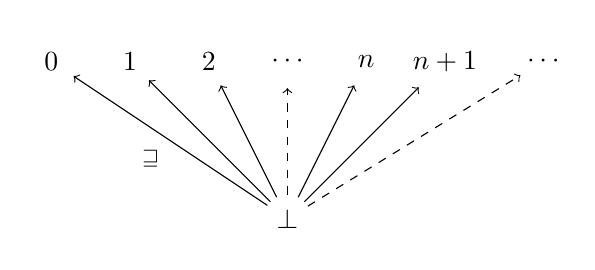
\begin{tikzpicture}[shorten >=1pt,->]
      \tikzstyle{vertex}=[circle,minimum size=17pt,inner sep=0pt]
      
      \node[vertex] (bot) at (3,0) {$\bot$};
      \node[vertex] (0) at (0,2) {$0$};
      \node[vertex] (1) at (1,2) {$1$};
      \node[vertex] (2) at (2,2) {$2$};
      \node[vertex] (dots) at (3,2) {$\cdots$};
      \node[vertex] (n) at (4,2) {$n$};
      \node[vertex] (n1) at (5,2) {$n+1$};
      \node[vertex] (ddots) at (6.25,2) {$\cdots$};
      
      \draw (bot) -- node[below left]{$\scriptstyle{\sqsupseteq}$} (0);
      \draw (bot) -- (1);
      \draw (bot) -- (2);
      \draw[dashed] (bot) -- (dots);
      \draw (bot) -- (n);
      \draw (bot) -- (n1);
      \draw[dashed] (bot) -- (ddots);
    \end{tikzpicture}    
    \caption{Графично представяне на $\sqsubseteq$ върху $\Nat_\bot$}
  \end{figure}
  \end{framed}
\end{example}

\begin{prop}
  \index{област на Скот!плоска}
  Нека $A$ е произволно множество и нека елементът $\bot \not \in A$.
  \marginpar{На англ. {\em flat domain}}
  Определяме наредената тройка $\A_\bot = (A_\bot, \sqsubseteq, \bot)$ като:
  \begin{itemize}
  \item 
    $A_\bot = A\cup\{\bot\}$;
  \item
    $\sqsubseteq$ задава {\em плоската наредба} върху $A_\bot$.
  \end{itemize}
  Тогава $\A_\bot$ е област на Скот, която ще наричаме {\bf плоска област на Скот} за множеството $A$.
\end{prop}


%%% Local Variables:
%%% mode: latex
%%% TeX-master: "../sep-notes"
%%% End:


\subsection{Крайно произведение}
\label{subsect:domains:product}
\index{област на Скот!крайно произведение}
\marginpar{\cite[стр. 125]{winskel}}

Нека $\A$ и $\B$ са области на Скот.
Тогава $\A \times \B \df (A \times B,\sqsubseteq,\bot)$, където
\begin{itemize}
\item
  $A \times B = \{\pair{a,b} \mid a \in A\ \&\ b \in B\}$;
\item
  $\pair{a,b} \sqsubseteq \pair{a',b'} \iff a \sqsubseteq^\A a'\ \&\ b \sqsubseteq^\B b'$;
\item
  $\bot = \pair{\bot^\A,\bot^\B}$.
\end{itemize}

\begin{framed}
  \begin{proposition}
    \label{pr:cartesian}
    Ако $\A$ и $\B$ са области на Скот, то $\A \times \B$ е област на Скот.
  \end{proposition}  
\end{framed}
\begin{hint}
  Лесно се съобразява, че $\sqsubseteq$ е частична наредба и че $\bot$ е най-малкият елемент.
  Да разгледаме една верига $\{\pair{a_i,b_i}\}^\infty_{i=1}$ в $\A \times \B$.
  Лесно се вижда, че
  \[\bigsqcup_i\pair{a_i,b_i} = \pair{\bigsqcup_ia_i,\bigsqcup_ib_i}.\]
  \begin{itemize}
  \item
    За произволен елемент $\pair{a_i,b_i}$ от веригата е ясно, че $a_i \sqsubseteq^\A \bigsqcup_ia_i$ и $b_i \sqsubseteq^\B \bigsqcup_i b_i$.
    Следователно, $\pair{\bigsqcup_ia_i,\bigsqcup_ib_i}$ е горна граница на веригата.
  \item
    Нека $\pair{c,d}$ е горна граница на веригата, т.е. за всяко $i$,
    $a_i \sqsubseteq^\A c$ и $b_i \sqsubseteq^\B d$.
    Но тогава $c$ е горна граница на веригата $\chain{a}{i}$ и следователно $\bigsqcup_ia_i \sqsubseteq^\A c$.
    Също така, $d$ е горна граница на веригата $\chain{b}{i}$ и следователно $\bigsqcup_i b_i \sqsubseteq^\B d$.
    Заключаваме, че $\pair{\bigsqcup_ia_i,\bigsqcup_ib_i} \sqsubseteq \pair{c,d}$, т.е. $\pair{\bigsqcup_ia_i,\bigsqcup_ib_i}$
    е точна горна граница на веригата.
  \end{itemize}
\end{hint}

Нека $\A_1,\dots,\A_n$, $n \geq 2$, са области на Скот. Дефинираме 
$\prod^n_{i=1}\A_i = (A, \sqsubseteq, \bot)$ по следния начин:
\begin{itemize}
\item
  Ако $n = 2$, то $\prod^2_{i=1} \A_i \df \A_1 \times \A_2$.
\item
  Ако $n > 2$, то $\prod^n_{i=1} \A_i \df (\prod^{n-1}_{i=1}\A_i) \times \A_n$.
\end{itemize}

Използвайки \Prop{cartesian}, лесно се съобразява следното твърдение.
\begin{proposition}
  Ако $\A_1,\dots,\A_n$, $n \geq 2$, са области на Скот, то $\prod^n_{i=1}\A_i$ е област на Скот.
\end{proposition}

\begin{framed}
  \begin{figure}[H]
    \centering
    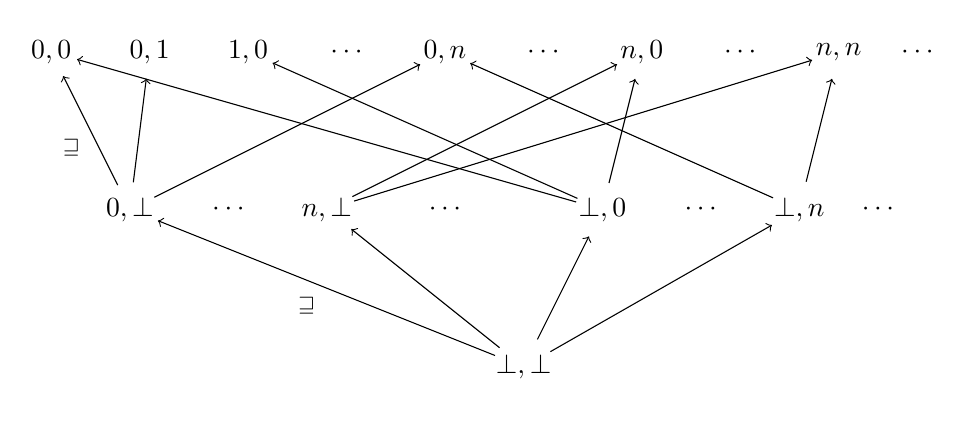
\begin{tikzpicture}[shorten >=1pt,->]
      \tikzstyle{vertex}=[circle,minimum size=17pt,inner sep=0pt]
      
      \node[vertex] (bot) at (5,-1) {$\pair{\bot,\bot}$};
      
      \node[vertex] (0b) at (0,1) {$\pair{0,\bot}$};
      \node[vertex] (db) at (1.25,1) {$\cdots$};
      \node[vertex] (nb) at (2.5,1) {$\pair{n,\bot}$};
      \node[vertex] (ddb) at (4,1) {$\cdots$};
      
      \node[vertex] (b0) at (6,1) {$\pair{\bot,0}$};
      \node[vertex] (bd) at (7.25,1) {$\cdots$};
      \node[vertex] (bn) at (8.5,1) {$\pair{\bot,n}$};
      \node[vertex] (bdd) at (9.5,1) {$\cdots$};
      
      \node[vertex] (00) at (-1,3) {$\pair{0,0}$};
      \node[vertex] (01) at (0.25,3) {$\pair{0,1}$};
      \node[vertex] (10) at (1.5,3) {$\pair{1,0}$};
      \node[vertex] (ddd) at (2.75,3) {$\cdots$};
      \node[vertex] (0n) at (4,3) {$\pair{0,n}$};
      \node[vertex] (dddd) at (5.25,3) {$\cdots$};
      \node[vertex] (n0) at (6.5,3) {$\pair{n,0}$};
      \node[vertex] (ddddd) at (7.75,3) {$\cdots$};
      \node[vertex] (nn) at (9,3) {$\pair{n,n}$};
      \node[vertex] (dddddd) at (10,3) {$\cdots$};

      \draw (bot) -- node[below left]{$\scriptstyle{\sqsupseteq}$} (0b);
      \draw (bot) -- (nb);
      \draw (bot) -- (b0);
      \draw (bot) -- (bn);

      \draw (0b) -- node[below left]{$\scriptstyle{\sqsupseteq}$} (00);
      \draw (0b) -- (01);
      \draw (0b) -- (0n);

      \draw (b0) -- (00);
      \draw (b0) -- (10);
      \draw (b0) -- (n0);
      \draw (nb) -- (n0);
      
      \draw (nb) -- (nn);
      \draw (bn) -- (0n);
      \draw (bn) -- (nn);

    \end{tikzpicture}    
    \caption{Графично представяне на част от $\sqsubseteq$ върху $\Nat^2_\bot$}
    \label{fig:flat-nat-2}
  \end{figure}
\end{framed}

Вижда се от \Fig{flat-nat-2}, че всяка верига в $\Nat^2_\bot$ има дължина най-много $3$.
Лесно се съобразява, че всяка верига в $\Nat^k_\bot$ има дължина най-много $k+1$.
Свойството, че всяка верига в $\Nat^k_\bot$ има само краен брой различни члена
ще се окаже важно по-нататък. Сега ще въведем понятие, което описва това свойство в произволна област на Скот.
\marginpar{ $\Nat^k_\bot = \underbrace{\Nat_\bot \times \cdots \times\Nat_\bot}_{k}$}

Нека $\A$ е област на Скот и да разгледаме една верига $\chain{a}{n}$ в $\A$.
Ще казваме, че $\chain{a}{n}$ се {\bf стабилизира}, ако съществува индекс $n_0$, за който
\[(\forall n \geq n_0)[a_{n_0} = a_{n}],\]
т.е.
\[a_0 \sqsubseteq a_1 \sqsubseteq a_2 \sqsubseteq \cdots \sqsubseteq a_{n_0} = a_{n_0+1} = a_{n_0+2} = \cdots\]
От казаното по-горе следва, че всяка растяща верига в $\Nat^k_\bot$ се стабилизира.

\marginpar{Едни от основните области на Скот, които ще разглеждаме при дефинирането на денотационната семантика ще бъдат $\Nat_\bot$ и $\Nat^k_\bot$.}


%%% Local Variables:
%%% mode: latex
%%% TeX-master: "../sep"
%%% End:


\section{Изображения в области на Скот}

\index{област на Скот!изображения}
Нека $\A_i = (A_i,\ \sqsubseteq_i,\ \bot_i)$, за $i = 1,2$, са области на Скот.
Ще въведем няколко основни видове изображения между $\A_1$ и $\A_2$, 
които ще използваме често. След това ще разгледаме свойства на тези изображения
и ще видим каква е връзката между тях.
\begin{itemize}
\item
  Всяка тотална функция от вида $f:A_1 \to A_2$ ще наричаме изображение между областите на Скот $\A_1$ и $\A_2$
  и ще записваме $f:\A_1 \to \A_2$.
  \marginpar{Тук $\bm{\bot}$ е различно от $\bot$, макар и трудно да се различават графически. Освен това, $\A$ е различно от $A$.}
  Да въведем означението 
  \[\Mapping{\A_1}{\A_2} \df (\{f \mid f:\A_1 \to \A_2\},\ \sqsubseteq,\ \bm{\bot}),\]
  \marginpar{\todo Сами проверете, че така дефинираната релация $\sqsubseteq$ задава частична наредба, при положение, че $\sqsubseteq_2$ е частична наредба.}
  където имаме следната релация между изображенията $f,g:\A_1 \to \A_2$:
  \[f \sqsubseteq g \dfff (\forall a \in \A_1)[f(a) \sqsubseteq_2 g(a)].\]
  Също така, изображението $\bm{\bot}:\A_1 \to \A_2$ е дефинирано като
  \[(\forall a \in \A_1)[\bm{\bot}(a) = \bot_2].\]
\end{itemize}

На хаскел можем да дефинираме изображението $\bm{\bot}$ по следния начин:
\begin{haskellcode}
ghci> let bottom _ = undefined
\end{haskellcode}

\begin{framed}
  \begin{theorem}
    \label{th:all-mappings-is-domain}
    $\Mapping{\A_1}{\A_2}$ е област на Скот.
  \end{theorem}  
\end{framed}
\begin{proof}
  Нетривиалната част в доказателството е да проверим, че всяка верига $(f_i)^{\infty}_{i=0}$ в $\Mapping{\A_1}{\A_2}$
  притежава точна горна граница.
  % \marginpar{За по-кратко пишем $\bar{a}$ вместо $a_1,\dots,a_n$}
  Да разгледаме изображението $h:\A_1 \to \A_2$, където:
  \begin{equation}
    \label{eq:9}
    h(a) \df \bigsqcup \{f_i(a) \mid i \in \Nat\}.
  \end{equation}
  Ще докажем, че $h$ е тази точна горна граница.
  \begin{itemize}
  \item
    \marginpar{Това задължително трябва да се провери,
      защото например множеството $\{\bot, 0, 3\}$ \emph{няма} точна горна граница относно плоската наредба в $\Nat_\bot$.}
    Първо, трябва да се убедим, че дефиницията на $h$ е ,,смислена'', т.е. $h$ е тотална функция.
    Трябва да докажем, че за всяко $a\in \A_1$, точната горна граница 
    \[\bigsqcup\{f_i(a) \mid i \in \Nat\}\] съществува.
    Да фиксираме произволен елемент $a \in \A_1$.
    Получаваме следната верига в $\A_2$:
    \[f_0(a) \sqsubseteq f_1(a) \sqsubseteq f_2(a) \sqsubseteq \cdots \]
    Понеже $\A_2$ е област на Скот, то тази верига притежава точна горна граница в $\A_2$,
    която означачаваме като $\bigsqcup\{f_i(a) \mid i \in \Nat\}$, а според нашата дефиниция,
    това е точно $h(a)$.
    Това означава, че $h$ е тотална функция.
  \item
    Дотук имаме, че $h \in \Mapping{\A_1}{\A_2}$.
    Лесно се съобразява, че $h$ е горна граница на веригата $\chain{f}{i}$, защото за всеки елемент $a \in \A_1$
    и произволен индекс $k$,
    \[f_k(a) \sqsubseteq \bigsqcup\{f_i(a) | i \in \Nat\} \df h(a).\]
  \item
    Сега остава да проверим, че $h$ е точна горна граница, т.е. $h$ е най-малката измежду всички горни граници на 
    веригата $\chain{f}{i}$.
    Нека $g$ е друга горна граница на $\chain{f}{i}$. Това означава, че за всеки индекс $i$,
    $f_i \sqsubseteq g$. Следователно, за фиксирано $a \in \A_1$,
    $g(a)$ е горна граница за веригата $(f_i(a))^{\infty}_{i=0}$.
    Тогава е ясно, че за разглеждания елемент $a$,
    \[h(a) \df \bigsqcup\{f_i(a) \mid i\in\Nat\} \sqsubseteq g(a).\]
    Понеже елементът $a$ е прозиволен, получаваме, че $h \sqsubseteq g$.
  \item
    Доказахме, че $h$ е горна граница и че $h$ е най-малката измежду всички горни граници.
    Заключваме, че $h$ е {\em точната горна граница} на веригата $\chain{f}{i}$.
    \marginpar{Получаваме, че \[(\bigsqcup_if_i)(a) = \bigsqcup_i\{f_i(a)\}.\] Добре е да свикнете с тези означения, защото по-нататък ще ги използваме често.}
    С други думи,
    \[h = \bigsqcup_i f_i.\]
  \end{itemize}
\end{proof}

Завършваме с един важен частен случай на горната теорема.
\begin{framed}
  \begin{corollary}
    $\Mapping{\Nat^n_\bot}{\Nat_\bot}$ е област на Скот.
  \end{corollary}
\end{framed}


%%% Local Variables:
%%% mode: latex
%%% TeX-master: "../sep"
%%% End:


\subsection{Монотонни изображения}

\index{изображение!монотонно}
Да разгледаме областите на Скот $\A_1 = (A_1,\ \sqsubseteq_1,\ \bot_1)$ и $\A_2 =(A_2,\ \sqsubseteq_2,\ \bot_2)$.
Едно изображение $f:\A_1\to \A_2$ се нарича {\bf монотонно}, ако
\[(\forall a,a'\in\A_1)[a \sqsubseteq_1 a' \implies f(a) \sqsubseteq_2 f(a')].\]
Да въведем означението
\[\Mon{\A_1}{\A_2} \df (\{f: \A_1 \to \A_2 \mid f\text{ е мон. изобр.}\},\ \sqsubseteq,\ \bm{\bot}).\]

\begin{framed}
  \begin{theorem}\label{th:monotone-is-domain}
    $\Mon{\A_1}{\A_2}$ е област на Скот.
  \end{theorem}  
\end{framed}
\begin{hint}
  Да фиксираме една верига $\chain{f}{i}$ в $\Mon{\A_1}{\A_2}$. Трябва да докажем, че тази верига притежава точна горна граница,
  която е монотонно изображение.
  Да разгледаме същото изображение $h:\A_1 \to \A_2$ както в доказателството на \Th{all-mappings-is-domain}, като
  \[h(a) \df \bigsqcup \{f_i(a) \mid i \in \Nat\}.\]
  Оттам знаем, че $h$ е точна горна граница на веригата. 
  Остава да докажем, че $h \in \Mon{\A_1}{\A_2}$.
  Нека $a \sqsubseteq b$. Тогава, за всеки индекс $k$, понеже $f_k$ са монотонни изображения, получаваме следното:
  \begin{align*}
    f_k(a) & \sqsubseteq f_k(b)\\
           & \sqsubseteq \bigsqcup \{f_i(b) \mid i \in \Nat\} \df h(b).
  \end{align*}
  Това означава, че $h(b)$ е горна граница за веригата ${(f_i(a))}^{\infty}_{i=0}$.
  Заключаваме, че 
  \begin{align*}
    h(a) & \df \bigsqcup \{f_i(a) \mid i \in \Nat\}\\
         & \sqsubseteq \bigsqcup \{f_i(b) \mid i \in \Nat\} \df h(b).
  \end{align*}
\end{hint}

\begin{corollary}\label{cr:flat-monotone-is-domain}
  $\Mon{\Nat^n_\bot}{\Nat_\bot}$ е област на Скот.
\end{corollary}

Удобно е да имаме следващото свойство на монотонните изображения като отделно твърдение за да можем да го използваме наготово по-късно.
\begin{proposition}\label{pr:monotone-chain}
  Нека $f \in \Mon{\A}{\B}$ и $\chain{a}{i}$ е верига от елементи на $\A$.
  Тогава
  \[\bigsqcup_i f(a_i) \sqsubseteq f(\bigsqcup_i a_i).\]
\end{proposition}
\begin{proof}
  Понеже $f$ е монотонно, то ${(f(a_i))}^{\infty}_{i=0}$ е верига от елементи на $\B$
  и тя има точна горна граница.
  Достатъчно е да докажем, че $f(\bigsqcup_i a_i)$ е горна граница на веригата ${(f(a_i))}^{\infty}_{i=0}$.
  Но това е лесно.
  Понеже $a_i \sqsubseteq \bigsqcup_i a_i$ и $f$ е монотонно, то веднага получаваме, че
  $f(a_i) \sqsubseteq f(\bigsqcup_i a_i)$.
  Заключаваме, че $\bigsqcup_i f(a_i) \sqsubseteq f(\bigsqcup_i a_i)$.
\end{proof}

%%% Local Variables:
%%% mode: latex
%%% TeX-master: "../sep"
%%% End:


\subsection{Непрекъснати изображения}\index{изображение!непрекъснато}

\marginpar{На англ. {\em continuous}}
Едно изображение $f:\A_1\to \A_2$ се нарича {\bf непрекъснато}, ако са изпълнени свойствата:
\begin{itemize}
\item
  $f$ е монотонно изображение;
\item
  при всеки избор на верига $\chain{a}{i}$ в $\A_1$, то имаме равенството
  \marginpar{Понеже $\A_1$ е област на Скот знаем, че $\bigsqcup_i a_i \in \A_1$}
  \marginpar{Понеже $f$ е монотонно, то ${(f(a_i))}^{\infty}_{i=0}$ е верига.}
  \marginpar{$\bigsqcup_i f(a_i) \df \bigsqcup\{f(a_i) \mid i \in \Nat\}$}
  \[f(\bigsqcup_i a_i) = \bigsqcup \{f(a_i) \mid i \in \Nat\}.\]  
\end{itemize}
Да означим
\[\Cont{\A_1}{\A_2} \df (\{f: \A_1 \to \A_2 \mid f\text{ е непр. изобр.}\},\ \sqsubseteq,\ \bm{\bot}).\]

% \begin{framed}
%   \begin{prop}
%     \label{pr:continuous-is-monotone}
%     За произволни области на Скот $\A_1$ и $\A_2$, всяко непрекъснато изображение $f:\A_1 \to \A_2$ е монотонно, т.е.
%     \[\Cont{\A_1}{\A_2}\ \subseteq\ \Mon{\A_1}{\A_2}.\]
%   \end{prop}
% \end{framed}
% \begin{proof}
%   Нека $f \in \Cont{\A_1}{\A_2}$.
%   Да вземем два произволни елемента в $\A_1$, за които $a \sqsubseteq_1 b$.
%   Ще докажем, че $f(a) \sqsubseteq_2 f(b)$.
%   Да разгледаме веригата $\chain{a}{i}$ в $\A_1$, където:
%   \[\underbrace{a_0}_{a} \sqsubseteq \underbrace{a_1}_{b} = \underbrace{a_2}_{b} = \underbrace{a_3}_{b} = \cdots\]
%   Ясно е, че 
%   \[\bigsqcup\{a_i \mid i \in \Nat\} = \bigsqcup\{a,b\} = b.\]
%   Тогава от непрекъснатостта на $f$ имаме, че
%   \begin{align*}
%     f(a) & = f(a_0) & \comment{\text{защото }a_0 \df a}\\
%     & \sqsubseteq_2 \bigsqcup\{f(a_i) \mid i \in \Nat\} & \comment{\text{защото }f(a_0) \in \{f(a_i) \mid i\in\Nat\}}\\
%     & = f(\bigsqcup_i a_i) & \comment{\text{защото $f$ е непр.}}\\
%     & = f(\bigsqcup\{a,b,b,b,\dots\}) & \comment{\text{от избора на веригата }\chain{a}{i}}\\
%     & = f(b) & \comment{\text{защото }a \sqsubseteq_1 b}.
%   \end{align*}
%   Така получихме, че за произволни $a,b\in\A_1$, 
%   \[a \sqsubseteq_1 b \implies f(a) \sqsubseteq_2 f(b).\]
% \end{proof}

Ясно е, че всяко непрекъснато изображение е монотонно.
Ествено е да си зададем въпроса дали имаме и обратното включване.
Оказва се, че в общия случай не е вярно, че всяко монотонно изображение е непрекъснато.

\begin{proposition}
  Съществува област на Скот $\A$, за която
  \[\Cont{\A}{\A} \subsetneqq \Mon{\A}{\A}.\]
\end{proposition}
\begin{hint}
  Нека $A = \{a_n \mid n \in \Nat\} \cup \{a_\omega, b_0\}$.
  Да разгледаме областта на Скот $\A = (A, \sqsubseteq, a_0)$, където 
  наредбата между елементите е следната:
  \[a_0 \sqsubseteq a_1 \sqsubseteq \cdots \sqsubseteq a_n \sqsubseteq \cdots \sqsubseteq a_\omega \sqsubseteq b_0. \]
  Нека $f(a_n) = a_{n+1}$, $f(a_{\omega}) = b_0$ и $f(b_0) = b_0$.
  Очевидно е, че $f$ е монотонно изображение.
  Лесно се вижда, че $f$ не е непрекъснато изображение, 
  защото
  \[f(\bigsqcup_n a_n) = f(a_\omega) = b_0,\]
  но 
  \[\bigsqcup_n f(a_n) = \bigsqcup_n a_{n+1} = a_\omega.\]
\end{hint}

Сега да видим един важен за нас случай, при който имаме и обратното включване.

\begin{framed}
  \begin{proposition}\label{pr:stab-continuous}
    Ако всяка верига в $\A_1$ се {\em стабилизира}, то
    \[\Mon{\A_1}{\A_2} \subseteq \Cont{\A_1}{\A_2}.\]
  \end{proposition}
\end{framed}
\begin{hint}
  Да разгледаме една верига $\chain{a}{i}$ в $\A_1$ и $f \in \Mon{\A_1}{\A_2}$.
  Ще докажем, че \[f(\bigsqcup_i a_i) = \bigsqcup_i f(a_i).\]

  \begin{enumerate}[(1)]
  \item
    % \marginpar{Това включване е вярно за произволна област на Скот $\A_1$.}
    % Ясно е, че за всяко монотонно изображение $f$,
    % понеже $a_i \sqsubseteq \bigsqcup_i a_i$, то $f(a_i) \sqsubseteq f(\bigsqcup_i a_i)$.
    % Това означава, че $f(\bigsqcup_i a_i)$ е горна граница на веригата $(f(a_i))^\infty_{i=0}$ в $\A_2$
    % и следователно
    % \[\bigsqcup_i f(a_i) \sqsubseteq f(\bigsqcup_i a_i).\]
    От \Prop{monotone-chain} веднага получаваме, че
    \[\bigsqcup_i f(a_i) \sqsubseteq f(\bigsqcup_i a_i).\]
  \item
    За другата посока ще използваме свойството, че веригата $\chain{a}{i}$ се стабилизира.
    Нека $n_0$ е индекс, такъв че $(\forall k \geq n_0)[a_k = a_{n_0}]$.
    Това означава, че $\bigsqcup_i a_i = a_{n_0}$.
    Тогава
    \[f(\bigsqcup_i a_i) = f(a_{n_0}) \sqsubseteq \bigsqcup_i f(a_i).\]
  \end{enumerate}
  
  От $(1)$ и $(2)$ следва, че $f(\bigsqcup_i a_i) = \bigsqcup_i f(a_i)$.
\end{hint}

Понеже всяка верига в $\Nat^n_\bot$ се {\em стабилизира}, то
получаваме следното важно следствие.
\begin{framed}
\begin{corollary}\label{cr:monotone-is-continuous}
  $\Mon{\Nat^n_\bot}{\Nat_\bot} = \Cont{\Nat^n_\bot}{\Nat_\bot}$.
\end{corollary}  
\end{framed}

% От доказателството на (1) за \Prop{stab-continuous} можем да извлечем следното свойство,
% което ще ни бъде полезно по-нататък.
% \begin{proposition}\label{pr:monotone-chain}
%   За всяко изображение $f \in \Mon{\A}{\B}$ и всяка верига $\chain{a}{i}$, е изпълнено, че
%   \[\bigsqcup_i f(a_i) \sqsubseteq f(\bigsqcup_i a_i).\]
% \end{proposition}

Понеже от \Cor{flat-monotone-is-domain} имаме, че монотонните изображения образуват област на Скот, 
то директно получаваме следната важна теорема.

\begin{framed}
\begin{theorem}
  \label{th:continuous-is-domain}
  $\Cont{\Nat^n_\bot}{\Nat_\bot}$ е област на Скот.
\end{theorem}
\end{framed}
% \begin{proof}
%   От \Cor{monotone-is-continuous} имаме, че 
%   \[\Mon{\Nat^n_\bot}{\Nat_\bot} = \Cont{\Nat^n_\bot}{\Nat_\bot}.\]
%   От \Cor{flat-monotone-is-domain} имаме, че 
%   \[(\Mon{\Nat^n_\bot}{\Nat_\bot}, \sqsubseteq, \Omega^{(n)})\]
%   е област на Скот. 
%   Оттук директно получаваме, че 
%   \[(\Cont{\Nat^n_\bot}{\Nat_\bot}, \sqsubseteq, \Omega^{(n)})\] е област на Скот.
% \end{proof}


% \begin{prop}
%   \label{pr:composition}
%   \index{изображения!композиция}
%   Ако $f \in \Cont{\A}{B}$ и $g \in \Cont{\B}{\C}$, то $g \circ f \in \Cont{\A}{\C}$,
%   където \[(g\circ f)(a) \df g(f(a)).\]
% \end{prop}
% \begin{hint}
%   Нека $\chain{a}{i}$ е верига в $\A$.
%   Да обърнем внимание, че понеже $f \in \Cont{\A}{\B}$,
%   то $f$ е монотонно изображение и тогава $(f(a_i))^\infty_{i=0}$ е верига в $\B$.
%   Тогава:
%   \begin{align*}
%     (g \circ f)(\bigsqcup_i a_i) & = g(f(\bigsqcup_i a_i)) & \comment{\text{от деф.}}\\
%     & = g(\bigsqcup_i f(a_i)) & \comment{f \text{ е непр.}}\\
%     & = \bigsqcup_i g(f(a_i)) & \comment{g \text{ е непр.}}
%   \end{align*}
% \end{hint}

%%% Local Variables:
%%% mode: latex
%%% TeX-master: "../sep"
%%% End:


\section{Област на Скот от непрекъснати изображения}

Следващата теорема е важна, защото с нейна помощ се доказват много свойства на непрекъснатите изображения от по-висок ред.

\begin{theorem}\label{th:double-chain}
  \marginpar{\cite[стр. 127]{winskel}}
  \marginpar{\cite[стр. 178]{models-of-computation}}
  Нека $\A = (A,\sqsubseteq,\bot)$ да бъде област на Скот и нека множеството 
  \[\{a_{m,n} \mid m,n \in \Nat\}\] от елементи на $A$ притежава свойството, че 
  \[n \leq n^\prime\ \&\ m \leq m^\prime\ \Rightarrow\ a_{n,m} \sqsubseteq a_{n^\prime,m^\prime}.\]
  Тогава са изпълнени равенствата
  \[\bigsqcup_m(\bigsqcup_n a_{n,m}) = \bigsqcup_n(\bigsqcup_{m} a_{n,m}) = \bigsqcup_n a_{n,n}.\]
\end{theorem}
\begin{proof}
  Първо ще въведем някои означения.
  \begin{itemize}
  \item 
    Да фиксираме произволно $m$. Тогава множеството $\{a_{n,m} \mid n \in \Nat\}$ образува верига:
    \[a_{0,m} \sqsubseteq a_{1,m} \sqsubseteq a_{2,m} \sqsubseteq \cdots\]
    \marginpar{По дефиниция, всяка монотонно растяща редица в област на Скот притежава точна горна граница.}
    Следователно тя има точна горна граница $b_m \dff \bigsqcup \{a_{n,m} \mid n \in \Nat\}$.
  \item
    Аналогично, при фиксирано $n$, множеството $\{a_{n,m} \mid m \in \Nat\}$ образува верига:
    \[a_{n,0} \sqsubseteq a_{n,1} \sqsubseteq a_{n,2} \sqsubseteq \ldots,\]
    която притежава точна горна граница $c_n \dff \bigsqcup \{a_{n,m} \mid m \in \Nat\}$.
  \end{itemize}
  Това означава, че трябва да докажем следното:
  \[\bigsqcup_m b_m = \bigsqcup_n c_n = \bigsqcup_n a_{n,n}.\]
  \begin{enumerate}[1)]
  \item 
    Първо да съобразим, че множеството $\{b_m \mid m \in \Nat\}$ образува верига в $\A$ и следователно притежава точна горна граница $\bigsqcup_m b_m$.
    Нека да разгледаме произволни $m \leq m^\prime$.
    Тогава \[(\forall n)[a_{n,m} \sqsubseteq a_{n,m^\prime} \sqsubseteq \bigsqcup_k a_{k,m^\prime} = b_{m^\prime}].\]
    Следователно $b_{m^\prime}$ е горна граница на веригата $(a_{n,m})^{\infty}_{n=0}$ и понеже $b_m$ е точна горна граница на $(a_{n,m})^{\infty}_{n=0}$, то получаваме, че \[b_m \sqsubseteq b_{m^\prime}.\]
    Това означава, че $\chain{b}{m}$ е верига в $\A$ и тя притежава точна горна граница $\bigsqcup_m b_m$.  
  \item
    С подобни разсъждения можем да докажем, че множеството $\{c_n \mid n \in \Nat\}$ образува верига в $\A$, която притежава точна горна граница $\bigsqcup_n c_n$.
  \item
    Сега ще докажем, че \[\bigsqcup_m b_m = \bigsqcup_n c_n.\]
    Имаме, че 
    \[(\forall m)(\forall n)[a_{n,m} \sqsubseteq \bigsqcup_{i}a_{i,m} = b_m \sqsubseteq \bigsqcup_i b_i],\]
    което е еквивалентно на 
    \[(\forall n)(\forall m)[a_{n,m} \sqsubseteq b_m \sqsubseteq \bigsqcup_i b_i].\]
    Да фиксираме произволно $n$.
    Тогава $\bigsqcup_i b_i$ е горна граница на веригата $(a_{n,i})^\infty_{i=0}$.
    Следователно, $c_n = \bigsqcup_i a_{n,i} \sqsubseteq \bigsqcup_i b_i$.
    Така получаваме, че $\bigsqcup_i b_i$ е горна граница и на веригата $\chain{c}{n}$
    и тогава \[\bigsqcup_n c_n \sqsubseteq \bigsqcup_i b_i.\]
    С аналогични разсъждения можем да докажем също, че 
    \[\bigsqcup_m b_m \sqsubseteq \bigsqcup_n c_n.\]
    Така доказахме, че \[\bigsqcup_m b_m = \bigsqcup_n c_n.\]
  \item
    Достатъчно е още да докажем, че
    \[\bigsqcup_n a_{n,n} = \bigsqcup_n c_n.\]
    Ясно е, че $a_{n,n}$ е елемент на веригата ${(a_{n,m})}^{\infty}_{m=0}$ и следователно
    $a_{n,n} \sqsubseteq \bigsqcup_m a_{n,m} = c_n \sqsubseteq \bigsqcup_n c_n$.
    Получаваме, че $\bigsqcup_n c_n$ е горна граница на веригата ${(a_{n,n})}^{\infty}_{n=0}$
    и следователно $\bigsqcup_n a_{n,n} \sqsubseteq \bigsqcup_n c_n$.
    
    За другата посока, да разгледаме произволен елемент $a_{n,m}$.
    Нека $k = \max\{n,m\}$.
    Ясно е, че $a_{n,m} \sqsubseteq a_{k,k} \sqsubseteq \bigsqcup_n a_{n,n}$.
    Следователно, $\bigsqcup_n a_{n,n}$ е горна граница на верига ${(a_{m,n})}^{\infty}_{m=0}$
    и оттук получаваме, че за всяко $n$, $c_n \sqsubseteq \bigsqcup_n a_{n,n}$.
    Получаваме, че $\bigsqcup_n a_{n,n}$ е горна граница на веригата $\chain{c}{n}$ и следователно
    $\bigsqcup_n c_n \sqsubseteq \bigsqcup_n a_{n,n}$.
  \end{enumerate}
  С това доказателството на теоремата е завършено.
\end{proof}

\begin{framed}
  \begin{lemma}
    Нека $\A$ и $\B$ са области на Скот.
    Нека $\chain{f}{k}$ е верига от елементи на $\Cont{\A}{\B}$.
    Да дефинираме изображението $h$ на $\A$ в $\B$ по следния начин
    \[h(a) \dff \bigsqcup\{f_k(a) \mid k \in \Nat\}.\]
    Изображението $h$ е {\em непрекъснато} и е {\em точна горна граница} на веригата $\chain{f}{k}$,
    т.е. $h = \bigsqcup_k f_k$.
  \end{lemma}
\end{framed}
\marginpar{Ако $b_k = f_k(a)$, то $h(a)$ е точната горна граница на веригата $\chain{b}{k}$ в $\B$}
\begin{proof}
  \ifhints
  Доказателството, че $h$ е точна горна граница на веригата $\chain{f}{k}$ е лесно.
  \begin{itemize}
  \item 
    Да разгледаме произволен елемент $a \in A$.
    Лесно се вижда, че понеже $\chain{f}{k}$ е верига, то $(f_k(a))^\infty_{k=0}$ също е верига.
    Това е така, защото всяко непрекъснато изображение е също така и монотонно.

    \marginpar{$\bigsqcup_n f_n(a)$ е съкратен запис за $\bigsqcup\{f_n(a) \mid n \in \Nat\}$.}
    Получаваме, че за всяко $k$, $f_k(a) \sqsubseteq^\B \bigsqcup_n f_n(a) \dff h(a)$.
    Понеже това е вярно за произволно $a \in A$, $(\forall k)[f_k \sqsubseteq h]$,
    което означава, че $h$ е горна граница на веригата.
  \item
    Да разгледаме произволно изображение $g$, което е горна граница на веригата $\chain{f}{k}$.
    За произволен елемент $a \in A$, 
    \[(\forall k)[f_k(a) \sqsubseteq^\B g(a)].\]
    Това означава, че $g(a)$ е горна граница на веригата ${(f_k(a))}^\infty_{k=0}$.
    Понеже $h(a) = \bigsqcup_k \{f_k(a)\}$ е точната горна граница на веригата ${(f_k(a))}^\infty_{k=0}$,
    то $h(a) \sqsubseteq^\B g(a)$.
    Оттук следва, че $h \sqsubseteq g$.
  \end{itemize}
  \fi
  По-сложната част на доказателството е проверката, че $h$ е непрекъснато изображение.
  Да вземем една монотонно растяща редица $\chain{a}{k}$ от елементи на $A$.
  \marginpar{За момента дори не е ясно дали $\{h(a_k) \mid k \in \Nat\}$ е верига в $\B$}
  Ще докажем, че \[h(\bigsqcup_k a_k) = \bigsqcup_k \{h(a_k)\}.\]
  Нека $e_{n,m} \dff f_n(a_m)$.
  Понеже всяко $f_n$ е непрекъснато и следователно монотонно изображение, то имаме
  \[n \leq n^\prime\ \&\ m \leq m^\prime\ \Rightarrow\ e_{n,m} \sqsubseteq^{\B} e_{n^\prime,m^\prime}.\]
  Следователно,
  \begin{align*}
    h(\bigsqcup_m a_m) & = \bigsqcup_n(f_n(\bigsqcup_m a_m)) & \comment{\text{от деф. на }h}\\
                       & = \bigsqcup_n(\bigsqcup_m f_n(a_m)) & \comment{\text{ защото } f_n \text{ е непр.}}\\
                       & = \bigsqcup_n(\bigsqcup_m e_{n,m}) = \bigsqcup_m(\bigsqcup_n e_{n,m}) & \comment{\text{от \Th{double-chain}}}\\
                       & = \bigsqcup_m(\bigsqcup_n f_n(a_m)) & \comment{\text{от деф. на }e_{n.m}}\\
                       & = \bigsqcup_m \{h(a_m)\}. & \comment{\text{от деф. на }h}
  \end{align*}
\end{proof}

Да напомним, че релацията $\sqsubseteq$ между две изображения е дефинирана като
\[f \sqsubseteq g \dfff (\forall a\in A)[f(a) \sqsubseteq^\B g(a)].\]
\begin{framed}
  \begin{theorem}
    \label{th:continuous-domain}
    Ако $\A$ и $\B$ са области на Скот, то $\Cont{\A}{\B}$ е област на Скот.
  \end{theorem}
\end{framed}

Нека $\A_1,\dots,\A_n$ и $\A$ са области на Скот и да разгледаме $f: \A_1\times \dots \times \A_n \to \A$.
Казваме, че $f$ е {\bf непрекъснато изображение по $i$-тия аргумент}, ако 
за всяка верига $\chain{a}{k}$ в $\A_i$, то
\[f(b_1,\dots, b_{i-1}, \bigsqcup_k a_k, b_{i+1},\dots,b_n) = \bigsqcup_k f(b_1,\dots, b_{i-1}, a_k, b_{i+1},\dots,b_n).\]

\begin{proposition}
  \label{pr:continuous-arguments}
  \marginpar{\cite[стр. 184]{models-of-computation}}
  Нека $\A_1,\dots,\A_n$ и $\A$ са области на Скот. Едно изображение
  \[f: \A_1\times \dots \times \A_n \to \A\]
  е непрекъснато точно тогава, когато $f$ е непрекъснато по всеки от аргументите си.
\end{proposition}
\begin{proof}
  \marginpar{\writedown Обобщете това твърдение за $n > 2$.}
  За по-просто изложение, да разгледаме случая $n = 2$.

  $(\Rightarrow)$ Лесно се съобразява, че ако $f$ е непрекъснато изображение, то $f$ е непрекъснато по всеки от аргументите си.
  Да видим например защо $f$ е непрекъснато по първия аргумент.
  Да разгледаме веригата ${(\pair{a_i,b})}^\infty_{i=0}$ от елементи на $\A\times\B$, за някое фиксирано $b$.
  Знаем, че $\bigsqcup_i \pair{a_i,b} = \pair{\bigsqcup_ia_i,b}$.
  Тогава
  \marginpar{Формално погледнато, правилно е да пишем $f(\pair{a,b})$ вместо $f(a,b)$.}
  \begin{align*}
    f(\bigsqcup_i a_i,b) & = f(\bigsqcup_i\pair{a_i,b}) \\
                        & = \bigsqcup_i f(a_i,b) & \comment{f\text{ е непрекъснато}}.
  \end{align*}
    
  $(\Leftarrow)$ Нека сега $f$ е непрекъснато по всеки от аргументите си. Ще докажем, че $f$ е непрекъснато.
  Нека ${\{\pair{a_n,b_n}\}}^\infty_{n=0}$ е верига в $\A_1\times \A_2$.
  Понеже от \Prop{cartesian} знаем, че
  \[\bigsqcup_n\pair{a_n,b_n} = \pair{\bigsqcup_n a_n,\bigsqcup_n b_n},\]
  ще докажем, че 
  \[\bigsqcup_n f(a_n,b_n) = f(\bigsqcup_n a_n,\bigsqcup_n b_n).\]
  Да положим $e_{n,m} = f(a_n,b_m)$.
  Понеже $f$ е непрекъснато по всеки от аргументите си, лесно се вижда, че $f$
  е монотонно изображение по всеки от аргументите си. Следователно, 
  \[n \leq n^\prime\ \&\ m \leq m^\prime\ \Rightarrow\ e_{n,m} \sqsubseteq e_{n^\prime,m^\prime}.\]  
  Получаваме, че
  \begin{align*}
    \bigsqcup_n f(a_n,b_n) & = \bigsqcup_n e_{n,n} & \comment{\text{от опр. на }e_{n,m}}\\
                           & = \bigsqcup_n (\bigsqcup_m e_{n,m}) & \comment{\text{от \Th{double-chain}}}\\
                           & = \bigsqcup_n (\bigsqcup_m f(a_n,b_m)) & \comment{\text{от опр. на }e_{n,m}}\\
                           & = \bigsqcup_n f(a_n,\bigsqcup_m b_m) & \comment{f \text{ е непр. по втория си аргумент}}\\
                           & = f(\bigsqcup_n a_n,\bigsqcup_m b_m) & \comment{f \text{ е непр. по първия си аргумент}}.
  \end{align*}
\end{proof}


%%% Local Variables:
%%% mode: latex
%%% TeX-master: "../sep"
%%% End:


\section{Основни непрекъснати изображения}

Да започнем като първо да дефинираме следните {\em основни изображения}
\begin{align*}
  & \plus : \Nat^2_\bot \to \Nat_\bot\text{, където}\\
  & \plus(a,b) \df
    \begin{cases}
      a+b, & \text{ако }a,b \in \Nat\\
      \bot, & \text{ако }\bot \in \{a,b\}
    \end{cases}\\
  & \minus : \Nat^2_\bot \to \Nat_\bot\text{, където}\\
  & \minus(a,b) \df
    \begin{cases}
      0, & \text{ако }a,b \in \Nat\ \&\ a < b\\
      a-b, & \text{ако }a,b \in \Nat\ \&\ a \geq b\\
      \bot, & \text{ако }\bot \in \{a,b\}
    \end{cases}\\
  & \eq : \Nat^2_\bot \to \Nat_\bot\text{, където}\\
  & \eq(a,b) \df
    \begin{cases}
      1, & \text{ако }a = b\ \&\ a,b \in \Nat\\
      0, & \text{ако }a \neq b\ \&\ a,b \in \Nat\\
      \bot, & \text{ако }\bot \in \{a,b\}
    \end{cases}
\end{align*}

% \marginpar{Озн. $\Nat^+ \df \Nat \setminus \{0\}$}

\begin{problem}\label{prob:basic-operations:continuous}
  Докажете, че изображенията $\texttt{(+)}$, $\texttt{(-)}$ и $\texttt{(==)}$ са непрекъснати.
\end{problem}
\begin{hint}
  Понеже $\Mon{\Nat^n_\bot}{\Nat_\bot} = \Cont{\Nat^n_\bot}{\Nat_\bot}$,
  достатъчно е да докажете, че изображенията са монотонни.
\end{hint}


\begin{problem}
  Докажете, че за всяко $b \in \B$, изображението
  $\texttt{const}_b \in \Cont{\prod^n_{i=1}\A_i}{\B}$ е непрекъснато, където
  \[\texttt{const}_b(a_1,\dots,a_n) = b.\]
\end{problem}


\begin{problem}
  \label{prob:projection}
  Докажете, че за всяко $n$ и $i < n$, изображението
  $\texttt{proj}^n_i \in \Cont{\A^n}{\A}$, където
  \[\texttt{proj}^n_i(a_0,\dots,a_{n-1}) = a_i.\]
\end{problem}

% \begin{definition}
%   \label{def:if}
%   \index{if}
%   Нека $\A$ е област на Скот. Дефинираме следното изображение
%   \begin{align*}
%     & \texttt{if}:\Nat_\bot \times \A \times \A \to \A \text{, където}\\
%     & \texttt{if}(b, a_1,a_2) =
%       \begin{cases}
%         a_1, & \text{ако } b \in \Nat^+\\
%         a_2, & \text{ако } b = 0\\
%         \bot, & \text{ако } b = \bot.
%       \end{cases}
%   \end{align*}
% \end{definition}

\begin{problem}\label{prob:basic-operations:if}
  Докажете, че $\texttt{if} \in \Cont{\Nat_\bot \times \A \times \A}{\A}$, където
  \begin{align*}
    & \texttt{if}(b, a_1,a_2) =
      \begin{cases}
        a_1, & \text{ако } b \in \Nat^+\\
        a_2, & \text{ако } b = 0\\
        \bot, & \text{ако } b = \bot.
      \end{cases}
  \end{align*}
\end{problem}
\begin{hint}
  Докажете, че $\texttt{if}$ е непрекъснато изображение по всеки от аргументите си поотделно.
\end{hint}


\begin{proposition}
  \label{pr:composition}
  \index{изображение!композиция}
  Ако $f \in \Cont{\A}{B}$ и $g \in \Cont{\B}{\C}$, то $g \circ f \in \Cont{\A}{\C}$,
  където \[(g\circ f)(a) \df g(f(a)).\]
\end{proposition}
\begin{hint}
  Нека $\chain{a}{i}$ е верига в $\A$.
  Да обърнем внимание, че понеже $f \in \Cont{\A}{\B}$,
  то $f$ е монотонно изображение и тогава ${(f(a_i))}^\infty_{i=0}$ е верига в $\B$.
  Тогава:
  \begin{align*}
    (g \circ f)(\bigsqcup_i a_i) & = g(f(\bigsqcup_i a_i)) & \comment{\text{от деф.}}\\
    & = g(\bigsqcup_i f(a_i)) & \comment{f \text{ е непр.}}\\
    & = \bigsqcup_i g(f(a_i)) & \comment{g \text{ е непр.}}
  \end{align*}
\end{hint}

\begin{problem}
  \label{prob:composition:continuous}
  Докажете, че изображението
  \[\compose:\Cont{\B}{\C}\times\Cont{\A}{\B} \to \Cont{\A}{\C}\]
  е непрекъснато, където $\compose(f,g) = f\circ g$.
  С други думи, $\compose$ е елемент на областта на Скот
  \[\Cont{\Cont{\B}{\C}\times\Cont{\A}{\B}}{\Cont{\A}{\C}}.\]
\end{problem}
\begin{hint}
  Използвайте \Prop{continuous-arguments}.
\end{hint}

Композицията на две функции е стандартна операция в \texttt{хаскел}.
\begin{haskellcode}
ghci> :t (.)
(.) :: (b -> c) -> (a -> b) -> a -> c  
\end{haskellcode}




%%% Local Variables:
%%% mode: latex
%%% TeX-master: "../sep"
%%% End:



\begin{proposition}\label{pr:cartesian-product:pair-continuous}
  Нека $f \in \Cont{\A}{\B}$ и $g \in \Cont{\A}{\C}$.
  Тогава $h \in \Cont{\A}{\B\times\C}$, където
  \[h(a) \df \pair{f(a),g(a)}.\]
  В такъв случай ще означаваме $h = f \times g$.
\end{proposition}
\begin{proof}
  Нека ${(a_i)}^{\infty}_{i=0}$ е верига в $\A$. Тогава:
  \begin{align*}
    h(\bigsqcup_i a_i) & = \pair{f(\bigsqcup_i a_i), g(\bigsqcup_i a_i)} & \comment{\text{от деф.}}\\
    & = \pair{\bigsqcup_i f(a_i), \bigsqcup_i g(a_i)} & \comment{\text{$f$ и $g$ са непр.}}\\
    & = \bigsqcup_i \pair{f(a_i),g(a_i)} & \comment{\text{от \Prop{cartesian}}}\\
    & = \bigsqcup_i h(a_i) & \comment{\text{от деф.}}
  \end{align*}
\end{proof}

% Обърнете внимание на следващото твърдение, защото ще го използваме често по-късно.
% То представлява обобщение на предишната задача и има сходно доказателство.
% Първо да въведем следното означение за произволно области на Скот $\B_1,\dots,\B_n$,
% \[\prod^n_{i=1}\B_i \df \B_1\times \B_2 \times \cdots \B_n,\]
% което също е област на Скот, дефинирана в {\em Раздел \ref{subsect:domains:product}}.

\begin{proposition}\label{pr:cartesian-product:general-continuous}
  Нека $f_i \in \Cont{\A}{\B_i}$, за $i = 1,\dots,n$.
  \marginpar{\writedown Докажете сами!}
  Тогава
  \[g \in \Cont{\A}{\prod^n_{i=1}\B_i},\]
  където
  \[g(a) \df \pair{f_1(a),f_2(a),\dots,f_n(a)}.\]
  В такъв случай ще означаваме $g = f_1\times f_2 \cdots \times f_n$.
\end{proposition}

\begin{proposition}\label{pr:cartesian-product:operator-continuous}
  Докажете, че изображението
  \[\texttt{cross}: \Cont{\A}{\B}\times\Cont{\A}{\C} \to \Cont{\A}{\B\times\C}\]
  е непрекъснато, където
  \[\texttt{cross}(f,g) = f \times g.\]
\end{proposition}


\begin{definition}\label{def:eval}\index{eval}
  Нека $\D$ и $\E$ са области на Скот. Дефинираме изображението 
  \[\texttt{eval}: \Cont{\D}{\E} \times \D \to \E,\]
  по следния начин:
  \[\texttt{eval}(f,d) \df f(d).\]  
\end{definition}

\begin{problem}\label{prob:eval}
  \marginpar{\cite[стр. 186]{models-of-computation}}
  Докажете, че $\texttt{eval}$ е непрекъснато изображение, т.е.
  \[\texttt{eval} \in \Cont{\Cont{\D}{\E} \times \D}{\E}.\]
\end{problem}
\begin{proof}
  Според \Prop{continuous-arguments}, достатъчно е да докажем, че $\texttt{eval}$ е непрекъснато
  изображение по всеки от двата си аргумента поотделно.
  
  Първо, нека $\chain{f}{n}$ е верига от елементи на $\Cont{\D}{\E}$ и $d$ е произволен елемент на $\D$.
  Тогава
  \[\texttt{eval}(\bigsqcup_n f_n,d) = (\bigsqcup_n f_n)(d) = \bigsqcup_n \{f_n(d)\} = \bigsqcup_n \texttt{eval}(f_n,d),\]
  т.е. изображението $\texttt{eval}$ е непрекъснато по първия си аргумент.
  
  Нека сега $\chain{d}{n}$ е верига от елементи на $\D$.
  Тогава за произволен елемент $f$ на $\Cont{\D}{\E}$ получаваме, че
  \[\texttt{eval}(f,\bigsqcup_n d_n) = f(\bigsqcup_n d_n) = \bigsqcup_n \{f(d_n)\} = \bigsqcup_n \texttt{eval}(f,d_n).\]
\end{proof}

%%% Local Variables:
%%% mode: latex
%%% TeX-master: "../sep"
%%% End:


\begin{problem}
  \marginpar{\cite[стр. 187]{models-of-computation}}
  Да разгледаме следното изображение
  \[\curry:\Mapping{\A\times \B}{\C} \to \Mapping{\A}{\Mapping{\B}{\C}},\]
  дефинирано като
  \[\curry(f)(a)(b) \dff f(a,b).\]
  Докажете, че ако $f$ е непрекъснато изображение, то
  $\curry(f)$ е непрекъснато изображение,
  т.е. $curry(f) \in \Cont{\A}{\Mapping{\B}{\C}}$.
\end{problem}
\begin{proof}
  Да разгледаме произволна верига $\chain{a}{i}$ от елементи на $\A$.
  Трябва да докажем, че
  \[\curry(f)(\bigsqcup_i a_i) = \bigsqcup_i \curry(f)(a_i).\]
  За целта, да разгледаме произволен елемент $b \in \B$. Тогава
  \begin{align*}
    \curry(f)(\bigsqcup_i a_i)(b) & = f(\bigsqcup_i a_i,b) & \comment\text{опр. на }\curry\\
                                  & = \bigsqcup_i f(a_i,b) & \comment\text{ $f$ е непр. по първия аргумент}\\
                                  & = \bigsqcup_i \{\curry(f)(a_i)(b)\}. & \comment\text{опр. на }\curry
  \end{align*}
\end{proof}

% \begin{hint}
%   Трябва да докажем, че
%   \[\texttt{curry}(\bigsqcup_i f_i)(a)(b) = \bigsqcup_i \{\texttt{curry}(f_i)(a,b)\}.\]
%   \begin{align*}
%     \texttt{curry}(\bigsqcup_i f_i)(a)(b) = (\bigsqcup_i f_i)(a,b)
%   \end{align*}
% \end{hint}


%%% Local Variables:
%%% mode: latex
%%% TeX-master: "../sep"
%%% End:


% \begin{definition}\label{def:if}\index{if}
  Нека $\A$ е област на Скот. Дефинираме следното изображение
  \begin{align*}
    & \texttt{if}:\Nat_\bot \times \A \times \A \to \A \text{, където}\\
    & \texttt{if}(b, a_1,a_2) =
      \begin{cases}
        a_1, & \text{ако } b \in \Nat^+\\
        a_2, & \text{ако } b = 0\\
        \bot, & \text{ако } b = \bot.
      \end{cases}
  \end{align*}
\end{definition}

\begin{problem}\label{prob:if}
  Докажете, че $\texttt{if}$ е непрекъснато изображение, т.е.
  \[\texttt{if} \in \Cont{\Nat_\bot \times \A \times \A}{\A}.\]
\end{problem}
\begin{hint}
  Докажете, че $\texttt{if}$ е непрекъснато изображение по всеки от аргументите си поотделно.
\end{hint}

%%% Local Variables:
%%% mode: latex
%%% TeX-master: "../sep"
%%% End:


\section{Най-малки неподвижни точки}\label{sect:lfp}\index{най-малка неподвижна точка}

\begin{itemize}
\item\index{неподвижна точка}
  Да фиксираме произволна област на Скот $\A = (A, \sqsubseteq, \bot)$ и да разгледаме едно изображение $f:\A\to\A$.
  Казваме, че $a \in \A$ е {\bf неподвижна точка} на $f$, ако $f(a) = a$.
\item\index{най-малка неподвижна точка}
  Казваме, че $a \in \A$ е {\bf най-малката неподвижна точка} на $f$, ако:
  \begin{itemize}
  \item 
    $a$ е неподвижна точка, т.е. $f(a) = a$;
  \item
    за всяко $b \in \A$ със свойството, че $f(b) = b$ имаме $a \sqsubseteq b$.
  \item
    \marginpar{least fixed point}
    Ще означаваме най-малката неподвижна точка на $f$ като $\lfp(f)$.
  \end{itemize}
\end{itemize}

\begin{framed}
\begin{theorem}[Клини]
  \label{th:knaster-tarski}
  \index{Клини}
  Нека $\A$ е област на Скот.
  Всяко $f \in \Cont{\A}{\A}$ притежава най-малка неподвижна точка.
\end{theorem}
\end{framed}
\begin{proof}
  \marginpar{В \cite{ditchev-soskov} се нарича теорема на Кнастер-Тарски. Според \href{https://en.wikipedia.org/wiki/Kleene_fixed-point_theorem}{уикипедия} е теорема на Клини. Теоремата на Кнастер-Тарски е по-силна и говори за монотонни изображения в решетки.}
  Определяме монотонно растяща редица от елементи на $\A$ по следния начин:
  \begin{align*}
    & a_0 \df \bot & \comment = f^0(\bot)\\
    & a_{n+1} \df f(a_n) & \comment = f^{n+1}(\bot).
  \end{align*}

  Първо ще докажем с индукция по $n$, че $\chain{a}{n}$ е верига.
  Ясно е, че $a_0 \sqsubseteq a_1$.
  Да приемем, че $a_n \sqsubseteq a_{n+1}$. Тогава, понеже всяко непрекъснато
  изображение е монотонно, то имаме, че
  \[\underbrace{f(a_n)}_{a_{n+1}} \sqsubseteq \underbrace{f(a_{n+1})}_{a_{n+2}}.\]

  Нека $a \df \bigsqcup_i a_i$. Тогава 
  \begin{align*}
    f(a) & = f(\bigsqcup_i a_i) & \comment a \df \bigsqcup_i a_i\\
         & = \bigsqcup_i f(a_i) & \comment f \text{ е непрекъсната}\\
         & = \bigsqcup_i a_{i+1} & \comment a_{i+1} = f(a_i)\\
         & = \bigsqcup_i a_i & \comment \text{защото }\chain{a}{i}\text{ е верига}\\
         & = a.
  \end{align*}
  Така доказахме, че $a$ е \emph{ неподвижна точка} на $f$.
  Остана да видим, че е най-малката неподвижна точка на $f$.

  Нека $b = f(b)$. С индукция по $n$ ще докажем, свойството $(\forall n)[a_n \sqsubseteq b]$.
  \begin{itemize}
  \item 
    За $n = 0$ е очевидно.
  \item
    Да приемем, че $a_n \sqsubseteq b$.
    Тогава $a_{n+1} \df f(a_n) \sqsubseteq f(b) = b$, защото $f$ е монотонно изображение.    
  \end{itemize}
  Така доказахме, че $b$ е горна граница на веригата $\chain{a}{n}$.
  Заключаваме, че $a \df \bigsqcup_n a_n \sqsubseteq b$.
  Следователно, $a$ е \emph{ най-малката неподвижна точка} на $f$,
  т.е. $a = \lfp(f)$.
\end{proof}

\begin{problem}
  Покажете, че съществува област на Скот $\A$ и изображение $f \in \Mon{\A}{\A}$, което притежава най-малка неподвижна точка, но тя не е $\bigsqcup_n f^n(\bot^\A)$.
\end{problem}
\ifhints\begin{hint}
  Вземете областта на Скот $\A$ и монотонното изображение $f$ както в \Prop{continuous-mappings-not-monotone}.
  % Да разгледаме $\A = (A,\ \sqsubseteq,\ a_0)$, където елементите на $A$ са подредени по следния начин:
  % \[A = \{ a_0 \sqsubset a_1 \sqsubset \cdots \sqsubset a_n \sqsubset \cdots \sqsubset a_\omega \sqsubset b \}.\]
  % т.е. $A$ е съставена от веригата ${(a_n)}^\infty_{n=0}$ веднага следвана от елементите $a_\omega$ и $b$.
  % Да обърнем внимание, че $\bigsqcup_n a_n = a_\omega$.
  % Сега да разгледаме изображението $f:\A\to\A$, където за всяко $n$,
  % \begin{align*}
  %   & f(a_n) = a_{n+1}\\
  %   & f(a_\omega) = b\\
  %   & f(b) = b.
  % \end{align*}
  % Лесно се вижда, че това изображение е монотонно.
  Лесно се вижда, че $f$ не е непрекъснато изображение, защото $\bigsqcup_n a_n = a_\omega$, и тогава:
  \[f(\bigsqcup_n a_n) = f(a_\omega) = b \neq a_\omega = \bigsqcup_n a_{n+1} = \bigsqcup_n \{f(a_n)\}.\]
  Според дефиницията на изображението $f$, единствената неподвижна точка на $f$ е елементът $b$.
  Това означава, че $b$ е също и най-малката неподвижна точка.
  \marginpar{Имаме, че $f^n(a_0) = a_n$.}
  Това е пример за монотонно изображение, което не е непрекъснато, но притежава най-малка неподвижна точка $b$,
  макар и тя да не е $a_\omega = \bigsqcup_n f^n(a_0)$.
\end{hint}
\fi

% \begin{problem}
%   Да разгледаме $\Gamma:\Partial{\Nat}{\Nat} \to \Partial{\Nat}{\Nat}$, където
%   \begin{enumerate}[a)]
%   \item
%     $\Gamma(f)(x) = 5$, за всяко $x \in \Nat$;
%   \item
%     $\Gamma(f)(x)$ не е деф. за всяко $x \in \Nat$;
%   \item
%     $\Gamma(f) = f$;
%   \item
%     $\Gamma(f) = f\circ f$;
%   \item
%     $\Gamma(f)(x) = x * f(x+1)$;
%     \item
%     $\Gamma(f)(x) =
%     \begin{cases}
%       \text{не е деф.}, & \text{ ако }x = 0\\
%       x * f(x-1), & \text{ ако }x > 0.
%     \end{cases}$    
%   \item
%     $\Gamma(f)(x) =
%     \begin{cases}
%       0, & \text{ ако }x = 0\\
%       x * f(x-1), & \text{ ако }x > 0.
%     \end{cases}$
%     \item
%     $\Gamma(f)(x) =
%     \begin{cases}
%       1, & \text{ ако }x = 0\\
%       x * f(x-1), & \text{ ако }x > 0.
%     \end{cases}$    
%   \end{enumerate}
% \end{problem}


% \newpage

% \begin{example}
%   Да разгледаме следното изображение $\Gamma:\Partial{\Nat}{\Nat} \to \Partial{\Nat}{\Nat}$, където
%   \[\Gamma(f)(x) \simeq
%     \begin{cases}
%       0, & \text{ ако }x = 0\\
%       x + f(x-1), & \text{ ако }x > 0.
%     \end{cases}\]
%   Първо да видим, че $\Gamma$ е монотонно изображение.
%   Нека $f \subseteq g$.
%   Трябва да докажем, че за всяко $x$, ако $\Gamma(f)(x) \simeq y$, то $\Gamma(g)(x) \simeq y$.
%   \begin{itemize}
%   \item
%     Нека $x = 0$.
%     Тогава $\Gamma(f)(0) \simeq 0 \simeq \Gamma(g)(0)$.
%   \item
%     Нека $x > 0$ и да приемем, че $\Gamma(f)(x) \simeq x + f(x-1) \simeq y$.
%     Това означава, че $f(x-1) \simeq z$, за някое $z$, и $x + z = y$.
%     От $f \subseteq g$ следва, че имаме също и $g(x-1) \simeq z$.
%     Тогава е ясно, че $\Gamma(g)(x) \simeq x + g(x-1) \simeq x+z = y$.
%   \end{itemize}
%   Разгледахме всички възмножни случаи за естественото число $x$ и
%   \marginpar{$\texttt{Graph}(\Gamma(f)) \subseteq \texttt{Graph}(\Gamma(g))$.}
%   видяхме, че за произволно $x$, ако $\Gamma(f)(x) \simeq y$, то $\Gamma(g)(x) \simeq y$.
%   Заключаваме, че $\Gamma(f) \subseteq \Gamma(g)$, т.е. $\Gamma$ е монотонно изображение.

%   Нека сега да видим, че $\Gamma$ е непрекъснато изображение.
%   Да разгледаме произволна верига $\chain{f}{i}$ от частични функции.
%   Трябва да докажем, че
%   \[\Gamma(\bigsqcup_i f_i) = \bigsqcup_i \Gamma(f_i).\]
%   Щом $\Gamma$ е монотонно, от \Prop{monotone-chain} вече знаем, че
%   \[\bigsqcup_i \Gamma(f_i) \subseteq \Gamma(\bigsqcup_i f_i).\]
%   Остава да докажем обратната посока. И така, нека първо да вземем $x = 0$.
%   Тогава $\Gamma(\bigsqcup_i f_i)(0) \simeq 0$. От дефиницията от $\Gamma$ знаем, че
%   за всяко $i$, $\Gamma(f_i)(0) \simeq 0$ и оттук $(\bigsqcup_i \Gamma(f_i))(0) \simeq 0$.
%   Следователно,
%   \[\Gamma(\bigsqcup_i f_i)(0) \simeq 0 \simeq (\bigsqcup_i \Gamma(f_i))(0).\]
%   Нека сега $x > 0$. Тогава
%   \marginpar{Да напомним, че $(\bigsqcup_i f_i)(u) \simeq v$ точно тогава, когато съществува индекс $i$, за който $f_i(u) = v$.}
%   \[\Gamma(\bigsqcup_i f_i)(x) \simeq x + (\bigsqcup_i f_i)(x-1) \simeq y.\]
%   Ясно е, че съществува $z$, за което $(\bigsqcup_i f_i)(x-1) \simeq z$ и $x + z = y$.
%   Знаем, че съществува индекс $i$, за който $f_i(x-1) \simeq z$.
%   Тогава, понеже $\Gamma(f_i)(x) \simeq x + f_i(x-1) \simeq x+z = y$, то следва, че $(\bigsqcup_i \Gamma(f_i))(x) \simeq y$.

%   Сега вече можем да намерим $\lfp(\Gamma) = \bigsqcup_n \Gamma^n(\bm{\bot})$.
%   Ще докажем, че
%   \[\lfp(\Gamma)(x) \simeq \frac{x(x+1)}{2}\] за всяко естествено число $x$.
%   Нека за улеснение да означим $g_n = \Gamma^n(\bm{\bot})$.
%   Ще докажем, че за всяко $n$,
%   \[g_n(x) \simeq \begin{cases}
%       \sum^x_{i=1}i, & \text{ ако } x < n\\
%       \text{не е деф.}, & \text{ ако } x \geq n.
%     \end{cases}\]
%   Ясно е, че $g_0 = \bm{\bot}$, което може да се запише и така:
%   \marginpar{Да напомним, че $\Gamma^0(g) = g$ и $\Gamma^{n+1}(g) = \Gamma(\Gamma^n(g))$.}
%   \[g_0(x) \simeq \begin{cases}
%       \sum^x_{i=1}i, & \text{ ако } x < 0\\
%       \text{не е деф.}, & \text{ ако } x \geq 0.
%     \end{cases}\]
%   Да приемем, че нашето твърдение е изпълнено за $g_n$.
%   Ще докажем, че то е изпълнено и за $g_{n+1}$. И така,
%   \begin{align*}
%     g_{n+1}(x) & \simeq= \Gamma(g_n)(x)\\
%                &  \simeq \begin{cases}
%                  0, & \text{ ако } x = 0\\
%                  x + g_n(x-1), & \text{ ако }x > 0\\
%                \end{cases}\\
%                & \stackrel{\text{И.П.}}{\simeq} \begin{cases}
%                  0, & \text{ ако } x = 0\\
%                  x + \sum^{x-1}_{i=1}i , & \text{ ако } 0 \leq x-1 < n\\
%                  \text{не е деф.}, & \text{ ако }x-1 \geq n\\
%                \end{cases}\\
%                & \simeq \begin{cases}
%                  0, & \text{ ако } x = 0\\
%                  \sum^{x}_{i=1}i , & \text{ ако } 1 \leq x < n+1\\
%                  \text{не е деф.}, & \text{ ако }x \geq n+1\\
%                \end{cases}\\
%                & \simeq \begin{cases}
%                  \sum^{x}_{i=1}i , & \text{ ако } x < n+1\\
%                  \text{не е деф.}, & \text{ ако }x \geq n+1.
%                \end{cases}
%   \end{align*}
%   Сега можем да заключим, че за всяко естествено число $x$,
%   \[g_{x+1}(x) \simeq \sum^x_{i=1}i = \frac{x(x+1)}{2}.\]
%   Тогава
%   \[\texttt{lfp}(\Gamma)(x) \simeq (\bigsqcup_i g_i)(x) \simeq \frac{x(x+1)}{2}.\]
% \end{example}

% Казваме, че елементът $a$ е {\bf преднеподвижна точка} на $f$,
% ако $f(a) \sqsubseteq a$.

\marginpar{Да се обясни къде се използва това твърдение.}
\begin{proposition}\label{pr:prefix-point}
  За всяко $f \in \Cont{\A}{\A}$ е изпълнено, че 
  \[(\forall a \in \Pref(f))[\lfp(f) \sqsubseteq a],\]
  където
  \index{преднеподвижна точка}
  \[\Pref(f) \df \{a \in \A \mid f(a) \sqsubseteq a\}\]
  е множеството от всички преднеподвижни точки на $f$.
  Това означава, че $\lfp(f)$ е най-малката преднеподвижна точка на $f$.
\end{proposition}
\begin{proof}
  Знаем от \hyperref[th:knaster-tarski]{Теоремата на Клини}, че $\lfp(f) = \bigsqcup_n f^n(\bot)$.
  Също така знаем, че $\chain{b}{n}$ е верига, където за улеснение сме положили $b_n \df f^n(\bot)$. 
  Ясно е също, че $\texttt{Pref}(f) \neq \emptyset$, защото $\lfp(f) \in \texttt{Pref}(f)$.
  Да фиксираме прозиволен елемент $a\in \texttt{Pref}(f)$.
  С индукция по $n$ ще докажем, че $b_n \sqsubseteq a$ за всяко $n$.
  \begin{itemize}
  \item 
    За $n = 0$ е очевидно, защото тогава $b_0 \df \bot \sqsubseteq a$.
  \item
    Да приемем, че $b_n \sqsubseteq a$.
    Ще докажем, че $b_{n+1} \sqsubseteq a$.
    Но това е лесно.
    \begin{align*}
      b_{n+1} & = f(b_n) & \comment \text{от деф. на }b_{n+1}\\
      & \sqsubseteq f(a) & \comment b_n \sqsubseteq a\ \&\ f\text{ е мон.}\\
      & \sqsubseteq a & \comment a \in \texttt{Pref}(f).
    \end{align*}
  \end{itemize}
  Така доказахме, че за всяко $n$, $b_n \sqsubseteq a$,
  откъдето следва, че $a$ е горна граница за веригата $\chain{b}{n}$, откъдето директно получаваме, че
  \[\lfp(f) = \bigsqcup_n b_n \sqsubseteq a.\]
\end{proof}

\begin{problem}
  Нека $\A$ е област на Скот и нека $f \in \Cont{\A}{\A}$.
  Да разгледаме множеството $B = \{a \in \A \mid f(a) = f\}$.
  Вярно ли е, че $\B = (B, \sqsubseteq, \lfp(f))$ е област на Скот.
  Обосновете се!
\end{problem}

\begin{problem}% Gunter textbook
  Нека $f \in \Cont{\A}{\A}$.
  Да разгледаме множеството 
  \[B = \{a \in \A \mid f(a) \sqsubseteq a\}.\]
  Вярно ли е, че 
  \[\B = (B, \sqsubseteq^\A, \lfp(f))\] е област на Скот?
  Обосновете се!
\end{problem}


\begin{problem} % Gunter textbook
  Да разгледаме множеството
  \[B = \{f \in \Mon{\A}{\A} \mid f\circ f = f\}.\]
  Вярно ли е, че 
  \[\B = (B,\ \sqsubseteq,\ \lambda x.\bot^\A)\] е област на Скот,
  където 
  \[f \sqsubseteq g \df (\forall a\in\A)[f(a) \sqsubseteq^\A g(a)] ?\]
  Обосновете се!
\end{problem}


\begin{problem}
  \label{prob:domains:lfp:compositon}
  \marginpar{Задача в Кеймбридж 2020 г. \cite{cambridge-website}}
  Нека $\A$ и $\B$ са области на Скот и нека $f \in \Cont{\A}{\B}$ и $g \in \Cont{\B}{\A}$.
  Докажете, че е изпълнено равенството:
  \[\lfp(f \circ g) = f(\lfp(g \circ f)).\]
\end{problem}

\begin{problem}
  \label{prob:domains:lfp:compositon-1}
  \marginpar{Изображения $h$, за които $h(\bot^\A) = \bot^\B$ се наричат точни. На англ. strict.}
  Нека $\A$ и $\B$ са области на Скот и нека $f \in \Cont{\A}{\A}$, $g \in \Cont{\B}{\B}$,
  и $h \in \Cont{\A}{\B}$, за които е изпълнено свойството, че $h \circ f = g \circ h \in \Cont{\A}{\B}$.
  Докажете, че ако $h$ е такава, че $h(\bot^{\A}) = \bot^\B$, то е изпълнено, че:
  \[\lfp(g) = h(\lfp(f)).\]
\end{problem}


%%% Local Variables:
%%% mode: latex
%%% TeX-master: "../sep"
%%% End:


% \subsection{Точни изображения}

\marginpar{На англ. се нарича {\em strict}. ,,Стандартната'' семантика на хаскел е {\em non-strict}}
\index{изображение!точно}
Едно изображение $f:\A^n_1 \to \A_2$ се нарича {\bf точно}, ако 
\[(\forall \bar{a}\in\A^n_1)[\bot_1\in\{a_1,\dots,a_n\} \implies f(a_1,\dots,a_n) = \bot_2].\]
% Тук ще разглеждаме съвкупността от точни изображения:
% \[S_n \dff \{f: \Nat^n_\bot \to \Nat_\bot \mid f\text{ е точна}\}.\]
За произволни области на Скот $\A_1$ и $\A_2$, ще означаваме съвкупността от
точните изображения като $\Strict{\A_1}{\A_2}$.

\begin{example}
  Да разгледаме свойствата на няколко прости изображения.
  \begin{itemize}
  \item 
    Изображението $f:\Nat_\bot \to \Nat_\bot$, дефинирано като 
    \[f(x) = 42,\]
    за всяко $x \in \Nat_\bot$,
    {\bf не е точно}, защото $f(\bot) = 42$. Лесно се вижда, че $f$ е монотонно и непрекъснато изображение.
  \item
    От друга страна, изображението $g:\Nat_\bot \to \Nat_\bot$, дефинирано като 
    \[g(x) = \bot,\]
    за всяко $x \in \Nat_\bot$, {\bf е точно}, защото $g(\bot) = \bot$.
    Освен това, $g$ е монотонно и непрекъснато изображение.
  \end{itemize}
\end{example}

Видяхме, че лесно се намират монотонни изображения, които не са точни.
Сега ще разгледаме обратната посока.

\begin{proposition}
  \label{pr:strict-is-monotone}
  Всяко точно изображение $f:\Nat^n_\bot \to \Nat_\bot$ е също така и монотонно.
  С други думи, 
  \[\Strict{\Nat^n_\bot}{\Nat_\bot} \subseteq \Mon{\Nat^n_\bot}{\Nat_\bot}.\]
\end{proposition}
\begin{proof}
  Нека $f$ е точно и $\bar{a} \sqsubseteq \bar{b}$.
  Ще проверим, че 
  \[f(\bar{a}) = c \sqsubseteq d = f(\bar{b}).\]
  \begin{itemize}
  \item 
    Ако $c = \bot$, то е очевидно, че $c \sqsubseteq d$.
  \item
    Интересният случай е когато $c \neq \bot$. Тогава трябва да видим, че $c = d$.
    Понеже $f$ е точна и $c \neq \bot$, това означава, че $\bot \not\in\{a_1,\dots,a_n\}$.
    Но понеже $\sqsubseteq$ е плоска наредба, и $\bar{a} \sqsubseteq \bar{b}$, това означава, че $\bar{a} = \bar{b}$.
    Следотвателно, наистина $c = d$.
  \end{itemize}
\end{proof}

\begin{framed}
  \begin{theorem}
    \label{th:strict-is-domain}
    $(\Strict{\Nat^n_\bot}{\Nat_\bot},\ \sqsubseteq,\ \bm{\bot}^{(n)})$ е област на Скот.
  \end{theorem}
\end{framed}
\begin{hint}
  Да разгледаме веригата $\chain{f}{i}$ от елементи на $\Strict{\Nat^n_\bot}{\Nat_\bot}$.
  Трябва да докажем, че тази верига притежава точна горна граница, която също е точно изображение.
  % Понеже от \Prop{strict-is-monotone} имаме, че всяка точна функция е монотонна, то наготово от 
  От доказателството на \Th{all-mappings-is-domain} знаем, че изображението $h$ дефинирано за всяко $\bar{a} \in \Nat^n_\bot$ като
  \[h(\bar{a}) \df \bigsqcup \{f_i(\bar{a}) \mid i \in \Nat\}\]
  е точна горна граница на веригата $\chain{f}{i}$.
  Остава да проверим, че $h$ е точно изображение.
  Нека $\bar{a} \in \Nat^n_\bot$ и да приемем, че $\bot \in \{a_1,\dots,a_n\}$.
  Тогава:
  \begin{align*}
    h(\bar{a}) & = \bigsqcup \{f_i(\bar{a}) \mid i \in \Nat\} & \comment{\text{от деф. на }h}\\
               & = \bigsqcup\{\bot,\bot,\dots,\bot,\dots\} & \comment{f_i\text{ са точни}}\\
               & = \bot.
  \end{align*}
\end{hint}

\begin{example}
  \label{ex:simple-non-continuous}
  Нека сега да разгледаме $h:\Nat_\bot \to \Nat_\bot$, където 
  \begin{align*}
    h(x) = &
    \begin{cases}
      0, & \text{ако }x = \bot,\\
      1, & \text{иначе}.
    \end{cases}
  \end{align*}
  Да видим колко ,,лошо'' изображение е $h$:
  \begin{itemize}
  \item 
    $h$ не е точно, защото $h(\bot) \neq \bot$;
  \item
    $h$ не е монотонно, защото $\bot \sqsubseteq 5$, но $h(\bot) = 0 \not\sqsubseteq 1 = h(5)$;
  \item
    $h$ не е непрекъснато, защото $\Cont{\Nat_\bot}{\Nat_\bot} = \Mon{\Nat_\bot}{\Nat_\bot}$.
  \end{itemize}
  Нека да видим, че хаскел не позволява такива ,,лоши'' функции:

  \begin{haskellcode}
ghci> let h(x) = if x == undefined then 0 else 1
ghci> h(5)
*** Exception: Prelude.undefined
ghci> h(undefined)
*** Exception: Prelude.undefined
  \end{haskellcode}
\end{example}

\begin{example}
  \label{ex:non-strict-monotone}
  Да разгледаме $f:\Nat^2_\bot \to \Nat_\bot$ дефинирано като \[f(x,y) = x.\]
  \begin{itemize}
  \item 
    $f$ не е точно, защото $f(0,\bot) = 0$.
  \item
    $f$ е монотонно, защото ако $\pair{x,y} \sqsubseteq \pair{x',y'}$, то $x \sqsubseteq x'$ и
    \[f(x,y) = x \sqsubseteq x' = f(x',y').\]
  \item
    $f$ е непрекъснато, защото от \Cor{monotone-is-continuous} знаем, че 
    $\Mon{\Nat^2_\bot}{\Nat_\bot} = \Cont{\Nat^2_\bot}{\Nat_\bot}$.
  \end{itemize}
\end{example}

Можем да обобщим всичко, което направихме дотук, със следната илюстрация на основните области на Скот, с които ще работим
в \Chapter{rec}.

\begin{framed}
    \begin{align*}
      \Strict{\Nat^n_\bot}{\Nat_\bot} & \subsetneqq \Mon{\Nat^n_\bot}{\Nat_\bot} & \comment{\text{от \Ex{non-strict-monotone} и \Prop{strict-is-monotone}}}\\
      & = \Cont{\Nat^n_\bot}{\Nat_\bot} & \comment{\text{от \Prop{continuous-is-monotone} и \Cor{monotone-is-continuous}}}\\
      & \subsetneqq \Mapping{\Nat^n_\bot}{\Nat_\bot} & \comment{\text{от \Ex{simple-non-continuous}}}.
    \end{align*}
\end{framed}

\begin{example}
  \label{ex:plus}
  Да разгледаме $f:\Nat^2_\bot \to \Nat_\bot$ дефинирана по следния начин:
  \[f(x,y) = 
  \begin{cases}
    \bot, & x = \bot\ \&\ y = \bot\\
    x, & x \neq \bot\ \&\ y = \bot\\
    y, & x = \bot\ \&\ y \neq \bot\\
    x+y, & x \neq \bot\ \&\ y \neq \bot.
  \end{cases}\]
  Изображението $f$ не е точно, защото например $f(\bot,0) \neq \bot$.
  $f$ не е монотонно изображение, защото $\pair{2,\bot} \sqsubseteq \pair{2,3}$, но $2 = f(2,\bot) \not\sqsubseteq f(2,3) = 5$.
  Също така, $f$ не е непрекъснато изображение, защото $\Mon{\Nat^2_\bot}{\Nat_\bot} = \Cont{\Nat^2_\bot}{\Nat_\bot}$.
\end{example}
% \begin{hint}
%   \begin{itemize}
%   \item 
%     $f$ не е точно изображение, защото например
%     $f(\bot,0) \neq \bot$.
%   \item
%     $f$ не е монотонно. Например,
%     \[\pair{\bot,0} \sqsubseteq \pair{1,0}\ \&\ f(\bot,0) = 0 \not\sqsubseteq 1 = f(1,0).\]    
%   \item
%     $f$ не е непрекъснато, защото $\Cont{\Nat^2_\bot}{\Nat_\bot} = \Mon{\Nat^2_\bot}{\Nat_\bot}$.
%   \end{itemize}    
% \end{hint}


% \subsection{Точни продължения}
% \index{изображение!точно продължение}

% Нека $A$ и $B$ са произволни множества, а $\A_\bot$ и $\B_\bot$ са плоските области на Скот получени съответно от $A$ и $B$.
% За еднa частична функция $f:A^n \to B$, определяме точното изображение $f^\star:\A^n_\bot \to \B_\bot$ по следния начин:
% \marginpar{$f^\star \in \Strict{\A^n_\bot}{\B_\bot}$}
% \begin{align*}
%   f^\star(\ov{a}) \dff
%   \begin{cases}
%     f(\ov{a}), & \text{ако }\bot\not\in\{a_1,\dots,a_n\}\ \&\ f(\ov{a})\text{ е деф.}\\
%     \bot, & \text{иначе}.
%   \end{cases}
% \end{align*}
% Изображението $f^\star$ се нарича {\bf точно продължение} на $f$.

% \begin{example}
%   Да разгледаме частичната функция $f:\Nat^2 \to \Nat$, дефинирана като
%   $f(x,y) = x+y$. Тогава точното продължение на $f$ е 
%   \[f^\star(x,y) = 
%   \begin{cases}
%     x+y, & x,y\in\Nat\\
%     \bot, & x = \bot \vee y = \bot.
%   \end{cases}\]
% \end{example}

% \Stefan{За какво ми е точното продължение да е непрекъснато?}
% \noindent Да дефинираме оператор $\Sigma^\star : \Partial{\Nat^n}{\Nat} \to \Strict{\Nat^n_\bot}{\Nat_\bot}$ като
% \[\Sigma^\star(f) = f^\star.\] 
% Ще наричаме $\Sigma^\star$ {\bf продължаващ} оператор, защото на всяка частична функция дава нейното точно продължение.

% \begin{framed}
%   \begin{prop}
%     $\Sigma^\star$ е непрекъснато изображение, т.е.
%     \[\Sigma^\star \in \Cont{\Partial{\Nat^n}{\Nat}}{\Strict{\Nat^n_\bot}{\Nat_\bot}}.\]
%   \end{prop}
% \end{framed}
% \begin{hint}
%   Трябва да докажем, че за произволна верига $(f_i)^{\infty}_{i=0}$ от частични функции, 
%   $\Sigma^\star(\bigcup_i f_i) = \bigsqcup_i \Sigma^\star(f_i)$.
%   \begin{itemize}
%   \item 
%     Лесно се съобразява, че ако $f \subseteq g$, то $\Sigma^\star(f) \sqsubseteq \Sigma^\star(g)$.
%     Оттук следва, че 
%     \[\bigsqcup_i \Sigma^\star(f_i) \sqsubseteq \Sigma^\star(\bigcup_i f_i).\]
%   \item
%     За другата посока,
%     Нека $\Sigma^\star(\bigcup_i f_i)(\ov{x}) = y \neq \bot$.
%     Това означава, че $\ov{x} \in \Nat^n$ и $(\bigcup_i f_i)(\ov{x}) \simeq y$.
%     Оттук следва, че съществува $i_0$, за което $f_{i_0}(\ov{x}) \simeq y$.
%     Тогава $\Sigma^\star(f_{i_0})(\ov{x}) = y$.
%     Понеже $y \neq \bot$, 
%     \[\bigsqcup_i (\Sigma^\star(f_i)(\ov{x})) = (\bigsqcup_i \Sigma^\star(f_i))(\ov{x}) = y.\]
%     Заключаваме, че $\Sigma^\star(\bigcup_i f_i)(\ov{x}) \sqsubseteq \bigsqcup_i (\Sigma^\star(f_i)(\ov{x}))$
%   \end{itemize}
% \end{hint}

% \Stefan{Това означава, че някъде трябва да се каже, че $\F_n$ е област на Скот. Някъде в тази глава трябва да е. Това може да бъде един от първите примери след дефиницията на О.С.}



%%% Local Variables:
%%% mode: latex
%%% TeX-master: "../sep"
%%% End:


% \subsection{Точни ограничения}
\index{изображение!точно ограничение}

Нека фиксираме две области на Скот $\A$ и $\B$.
За едно изображение $f \in \Mapping{\A^n}{\B}$, дефинираме точното изображение $f_\star \in \Strict{\A^n}{\B}$ по следния начин:
\[f_\star(\bar{a}) =
\begin{cases}
  f(\bar{a}), & \text{ако } \bot\not\in\{a_1,\dots,a_n\}\\
  \bot, & \text{ако }\bot\in\{a_1,\dots,a_n\}.
\end{cases}\]
Ще казваме, че $f_\star$ е {\bf точно ограничение} на $f$.

\begin{framed}
  \begin{prop}
    За всяко $f \in \Mapping{\A^n}{\B}$, имаме 
    \[f_\star \sqsubseteq f.\]
  \end{prop}
\end{framed}

\begin{example}
  Точното ограничение на функцията $f$ от \Ex{plus} е
  \[f_\star(x, y) =
  \begin{cases}
    x + y, & \text{ако } x \neq \bot\ \&\ y \neq \bot\\
    \bot, & \text{иначе}
  \end{cases}
\]
\end{example}

\begin{example}
  Да видим какъв резултат връща хаскел при следните извиквания:
  
  \begin{haskellcode}
ghci> (\x -> 5) 4
5
ghci> (\x -> 5) undefined
5
  \end{haskellcode}
  
  От второто извикване се вижда, че в хаскел, анонимната функция $\lambda x.5$ е дефинирана и върху $\bot$ и връща отново $5$.
  \marginpar{$(\lambda x.5)(4) = 5$, $(\lambda x.5)(\bot) = 5$}
  Това е естествено, понеже хаскел е {\em неточен} език, т.е. една функция може да има като аргумент $\bot$
  и да връща ,,смислен'' резултат. 

  \marginpar{Повече информация за \texttt{seq} може да се намери в \cite[стр. 108]{real-world-haskell}}
  При разглеждането на семантики на езици за програмиране, ще се нуждаем от това да направим една функция {\em точна}.
  Такава възможност има и в хаскел с командата \texttt{seq}.
  
  \begin{haskellcode}
ghci> :t seq
seq :: a -> b -> b
ghci> (\x -> x `seq` 5) 4
5
ghci> (\x -> x `seq` 5) undefined
*** Exception: Prelude.undefined
ghci> :set -XBangPatterns
ghci> (\(!x) -> 5) undefined
*** Exception: Prelude.undefined
\end{haskellcode}
  
  Командата \texttt{seq} приема два аргумента. Тя работи като оценява първия аргумент, като очаква той да се оцени до ,,смислен'' резултат, т.е. нещо различно от $\bot$. След това връща втория.
  Тук първия пример се превежда като $(\lambda x. 5)_\star(4) = 5$, а втория като $(\lambda x.5)_\star(\bot) = \bot$.
\end{example}

За произволно естествено число $n$, да дефинираме изображение
\[\Sigma_\star : \Mapping{\Nat^n_\bot}{\Nat_\bot} \to \Strict{\Nat^n_\bot}{\Nat_\bot},\]
където
\[\Sigma_\star(f) = f_\star.\] 
Ще наричаме $\Sigma_\star$ {\bf ограничаващ} оператор, защото на всяка функция дава нейното точно ограничение.

\begin{framed}
\begin{prop}
  \label{pr:strict-operator}
  За всяко $n$, $\Sigma_\star$ е непрекъснат оператор, т.е.
  \[\Sigma_\star \in \Cont{\Mapping{\Nat^n_\bot}{\Nat_\bot}}{\Strict{\Nat^n_\bot}{\Nat_\bot}}.\]
\end{prop}  
\end{framed}
\begin{hint}
  Трябва да докажем, че за произволна верига $\chain{f}{i}$ от елементи на $\Mapping{\Nat^n_\bot}{\Nat_\bot}$, имаме
  \[\Sigma_\star(\bigsqcup_i f_i) = \bigsqcup_i \Sigma_\star(f_i).\]
  \begin{enumerate}[(1)]
  \item 
    Лесно се съобразява, че $\Sigma_\star$ е монотонно изображение, т.е.
    \[f \sqsubseteq g \implies \Sigma_\star(f) \sqsubseteq \Sigma_\star(g).\]
    Сега използваме \Prop{monotone-chain}, откъдето следва, че
    \[\bigsqcup_i \Sigma_\star(f_i) \sqsubseteq \Sigma_\star(\bigsqcup_i f_i).\]
  \item
    За другата посока, нека да разгледаме $\ov{a}$, за които
    \marginpar{Случаят $\Sigma_\star(\bigsqcup_i f_i)(\ov{a}) = \bot$ е тривиален.}
    \[\Sigma_\star(\bigsqcup_i f_i)(\ov{a}) = b \neq \bot.\]
    Щом $b \neq \bot$, то ако $\ov{a} = (a_1, \dots, a_n)$, със сигурност $\bot \not\in \{a_1, \dots, a_n\}$.
    Тогава директно имаме, че $(\bigsqcup_i f_i)(\ov{a}) = b \neq \bot$.
    Сега от \Problem{sup-f} получаваме, че съществува $i_0$, за което $f_{i_0}(\ov{a}) = b$.
    Ясно е, че също така $\Sigma_\star(f_{i_0})(\ov{a}) = b$ и оттук
    $(\bigsqcup_i \Sigma_\star(f_i))(\ov{a}) = b$,
    защото $\Sigma_\star(f_{i_0}) \sqsubseteq \bigsqcup_i \Sigma_\star(f_i)$.
    Заключаваме, че
    \[\Sigma_\star(\bigsqcup_i f_i) \sqsubseteq \bigsqcup_i\Sigma_\star(f_i).\]
  \end{enumerate}
\end{hint}

%%% Local Variables:
%%% mode: latex
%%% TeX-master: "../sep-notes"
%%% End:



% \section{Оператор за най-малка неподвижна точка}

\begin{theorem}
  \marginpar{Доказателството в \cite[стр. 188]{models-of-computation} е малко по-различно.}
  % \index{$Y_\A$}
  Нека $\A$ е област на Скот и нека $f \in \Cont{\A}{\A}$.
  \marginpar{Знаем от \Th{knaster-tarski}, че най-малката неподвижна точка на $f$ е елемента $\bigsqcup_n f^n(\bot^\A)$.}
  Тогава изображението $\texttt{fix} : \Cont{\A}{\A} \to \A$, определено като
  \[Y(f) = \lfp(f),\]
  е непрекъснато, т.е.
  $Y \in \Cont{\Cont{\A}{\A}}{\A}$.
\end{theorem}
\begin{proof}
  Нека да вземем една верига $\chain{f}{n}$ от непрекъснати изображения.
  Нашата цел е да докажем, че
  \[Y(\bigsqcup_n f_n) = \bigsqcup_n \texttt{fix}(f_n).\]
  \marginpar{Записът ще стане много тромав, ако вместо $h$ използваме означението $\bigsqcup_n f_n$.}
  Да означим с $h$ точната горна граница на $\chain{f}{n}$.
  Знаем, че $h(a) = \bigsqcup_n \{f_n(a)\}$, а от \Th{continuous-domain} знаем, че $h$ е непрекъснато изображение.
  \begin{proposition}
    За всяко $k \geq 0$ и за всеки елемент $a \in \A$,
    \[h^k(a) = \bigsqcup_n \{f^k_n(a)\}.\]
  \end{proposition}
  \begin{proof}
    Ще докажем твърдението с индукция по $k$, като случая $k = 0$ е ясен, защото $h^0(a) = f^0_n(a) = a$.
    Нека приемем, че твърдението е вярно за произволно $k$.
    Ще докажем, че твърдението е вярно за $k+1$.
    \begin{align*}
      h^{k+1}(a) & = h(h^k(a)) & \\
                 & = h(\bigsqcup_n f^k_n(a))& \comment{\text{ от инд. предположение}}\\
                 & = \bigsqcup_n h(f^k_n(a))& \comment{h \text{ е непрекъснато изображение}}\\
                 & = \bigsqcup_n (\bigsqcup_m f_m(f^k_n(a))). & 
    \end{align*}
    
    Да положим $b_n = f^k_n(a)$, за всяко $n$.
    Понеже $f_n \sqsubseteq f_{n^\prime}$, лесно се съобразява, че за $n \leq n^\prime$
    имаме $b_n \sqsubseteq^\A b_{n^\prime}$.

    Сега да положим $e_{m,n} = f_m(b_n)$.
    Отново, понеже $\chain{b}{n}$ и $\chain{f}{m}$ са вериги, имаме 
    \[m \leq m^\prime\ \&\ n\leq n^\prime\ \Rightarrow\ e_{m,n} \sqsubseteq^\A e_{m^\prime,n^\prime}.\]
    Получаваме, че
    \begin{align*}
      h^{k+1}(a) & = \bigsqcup_n (\bigsqcup_m f_m(f^k_n(a))) & \comment{\text{ от горното равенство за } h^{k+1}}\\
                 & = \bigsqcup_n (\bigsqcup_m e_{m,n}) & \comment{\text{ от определението на }e_{m,n}}\\
                 & = \bigsqcup_n e_{n,n} & \comment{\text{ от \Th{double-chain}}}\\
                 & = \bigsqcup_n f_n(f^k_n(a))  = \bigsqcup_n f^{k+1}_n(a) & 
    \end{align*}
    С това твърдението е доказано.
  \end{proof}
  Сега вече сме готови да докажем непрекъснатостта на $Y$.
  Имаме, че:
  \begin{align*}
    Y(\bigsqcup_n f_n) & = Y(h) & \comment{\text{ от опр. на }h}\\
                       & = \bigsqcup_m h^m(\bot^\A) & \comment{\text{ от опр. на }Y }\\
                       & = \bigsqcup_m (\bigsqcup_n f^m_n(\bot^\A)) & \comment{\text{ от горното твърдение}}.
  \end{align*}
  
  Да положим $e_{m,n} = f^m_n(\bot^\A)$.
  Отново лесно се съобразява, че 
  \[m \leq m^\prime\ \&\ n\leq n^\prime\ \Rightarrow\ e_{m,n} \sqsubseteq^\A e_{m^\prime,n^\prime}.\]
  Получаваме, че
  \begin{align*}
    Y(\bigsqcup_n f_n) & = \bigsqcup_m (\bigsqcup_n f^m_n(\bot^\A)) & \comment{\text{ от горното равенство}}\\
                          & = \bigsqcup_m (\bigsqcup_n e_{m,n}) & \comment{\text{ от опр. на }e_{m,n}}\\
                          & = \bigsqcup_n(\bigsqcup_m e_{m,n}) & \comment{\text{ от \Th{double-chain}}}\\
                          & = \bigsqcup_n (\bigsqcup_m f^m_n(\bot^\A)) = \bigsqcup_n Y(f_n). & \comment{\text{ от опр. на }Y}.
  \end{align*}
\end{proof}

\marginpar{Добре е да погледнете това: \url{https://en.wikibooks.org/wiki/Haskell/Fix_and_recursion}}

\begin{haskellcode}
ghci> fact x = if x == 0 then 1 else x * fact(x-1)
ghci> fact 5
120
ghci> fix f = x where x = f x
ghci> :t f
fix :: (t -> t) -> t
ghci> fact' = fix \f x -> if x == 0 then 1 else x * f(x-1)
ghci> fact' 5
120
ghci> gamma f = \x -> if x == 0 then 1 else x * f(x-1)
ghci> :t gamma
(t -> t) -> t -> t
ghci> fact'' = fix gamma
ghci> fact'' 5
120
ghci> fix' f = x where x = f(f(f(x)))
ghci> fact''' = fix' gamma
ghci> fact''' 5
120
\end{haskellcode}


%%% Local Variables:
%%% mode: latex
%%% TeX-master: "../sep"
%%% End:



\section{Най-малко решение на система от уравнения}

\begin{problem}
  % \label{pr:cartesian-continuous}
  Нека $f \in \Cont{\A}{\B}$ и $g \in \Cont{\A}{\C}$.
  Докажете, че $h \in \Cont{\A}{\B\times\C}$, където
  \[h(a) \dff \pair{f(a),g(a)}.\]
  В такъв случай ще означаваме $h = f \times g$.
\end{problem}
\begin{proof}
  Нека $(a_i)^{\infty}_{i=0}$ е верига в $\A$. Тогава:
  \begin{align*}
    h(\bigsqcup_i a_i) & = \pair{f(\bigsqcup_i a_i), g(\bigsqcup_i a_i)} & \comment{\text{от деф.}}\\
    & = \pair{\bigsqcup_i f(a_i), \bigsqcup_i g(a_i)} & \comment{\text{$f$ и $g$ са непр.}}\\
    & = \bigsqcup_i \pair{f(a_i),g(a_i)} & \comment{\text{от \Prop{cartesian}}}\\
    & = \bigsqcup_i h(a_i) & \comment{\text{от деф.}}
  \end{align*}
\end{proof}

Обърнете внимание на следващото твърдение, защото ще го използваме често по-късно.
То представлява обобщение на предишната задача и има сходно доказателство.
% Първо да въведем следното означение за произволно области на Скот $\B_1,\dots,\B_n$,
% \[\prod^n_{i=1}\B_i \dff \B_1\times \B_2 \times \cdots \B_n,\]
% което също е област на Скот, дефинирана в {\em Раздел \ref{subsect:domains:product}}.

\begin{prop}
  \label{pr:product-continuous}
  Нека $f_i \in \Cont{\A}{\B_i}$, за $i = 1,\dots,n$.
  \marginpar{\writedown Докажете сами!}
  Тогава
  \[g \in \Cont{\A}{\prod^n_{i=1}\B_i},\]
  където
  \[g(a) \dff \pair{f_1(a),f_2(a),\dots,f_n(a)}.\]
  В такъв случай ще означаваме $g = f_1\times f_2 \cdots \times f_n$.
\end{prop}
Нека $\A_1,\dots,\A_n$ са области на Скот 
и да разгледаме изображенията
\[f_i:\prod^n_{k=1}\A_k \to \A_i,\] за $i = 1,\dots,n$.
\index{решение на система}
Казваме, че $\bar{a} = \pair{a_1,\dots,a_n}$ е {\bf решение на системата}

\begin{align*}
  \bigstar = 
  \begin{cases}
    &f_1(x_1,\dots,x_n) = x_1\\
    & \ \vdots\\
    & f_n(x_1,\dots,x_n) = x_n,
  \end{cases}
\end{align*}

ако са в сила равенствата 
\begin{align*}
  & f_1(a_1,\dots,a_n) = a_1\\
  & \ \vdots\\
  & f_n(a_1,\dots,a_n) = a_n.
\end{align*}
\index{решение на система!най-малко}

Казваме, че $\bar{a}$ е {\bf най-малкото решение} на системата $\bigstar$, ако за всяко друго решение $\bar{b}$
е изпълнено, че $\bar{a} \sqsubseteq \bar{b}$.

\begin{framed}
\begin{thm}
  \label{th:sep:min-solution-system}
  За произволни изображения $f_i \in \Cont{\prod^n_{k=1}\A_k}{\A_i}$, за $i = 1,\dots,n$, системата
  \begin{align*}
    & f_1(x_1,\dots,x_n) = x_1\\
    & \vdots\\
    & f_n(x_1,\dots,x_n) = x_n,
  \end{align*} 
  притежава най-малко решение.
\end{thm}
\end{framed}
\begin{proof}
  Първо да дефинираме както в \Prop{product-continuous} непрекъснатото изображение 
  \[g \dff f_1\times\dots\times f_n : \prod^n_{k=1}\A_k \to  \prod^n_{k=1}\A_k,\]
  като 
  \[g(\bar{a}) \dff \pair{f_1(\bar{a}),\dots,f_n(\bar{a})}.\]
  От \hyperref[th:knaster-tarski]{Теоремата на Клини} знаем, че $g$ притежава най-малка неподвижна точка
  $\bar{a} = \pair{a_1,\dots,a_n}$. Ще проверим, че $\ov{a}$ е най-малкото решение на системата.
  \begin{itemize}
  \item 
    Понеже $\ov{a}$ е неподвижна точка на $g$, то
    \begin{align*}
      g(a_1,\dots,a_n) & = \pair{f_1(\ov{a}),\dots,f_n(\ov{a})} & \comment{\text{от деф. на }g}\\
                       & = \pair{a_1,\dots,a_n} & \comment{\ov{a}\text{ е неподвижна точка}}.
    \end{align*}
    Оттук директно следва, че $f_i(\bar{a}) = a_i$, за $i = 1, \dots, n$, и следователно $\ov{a}$ е решение на системата.
  \item
    Нека $\ov{b} = \pair{b_1,\dots,b_n}$ е друго решение на системата, т.е. 
    $f_i(\ov{b}) = b_i$, за $i = 1, \dots, n$. Тогава 
    $g(\ov{b}) = \pair{f_1(\ov{b}),\dots,f_n(\ov{b})} = \ov{b}$.
    Следователно $\bar{b}$ е неподвижна точна на $g$.
    Понеже $\ov{a} = \lfp(g)$, то $\ov{a} \sqsubseteq \ov{b}$.
  \end{itemize}
  Така достигнахме до извода, че $\ov{a}$ е най-малкото решение на системата.
\end{proof}

Ще завършим този раздел с две твърдения, които ще улеснят нашите разсъждения при 
решаването на задачи.

\begin{framed}
  \begin{prop}
    \label{pr:system:independent}
    Да разгледаме изображенията $f \in \Cont{\A\times\B}{\A}$ и $g \in \Cont{\B}{\B}$,
    за които имаме системата от уравнения
    \begin{align*}
      \bigstar = 
      \begin{cases}
        & f(x,y) = x\\
        & g(y) = y.
      \end{cases}
    \end{align*}  
    Нека $b_0 = \lfp(g)$ и $a_0 = \lfp(\hat{f})$, където $\hat{f}(a) \df f(a,b_0)$.
    Тогава $\pair{a_0,b_0}$ е най-малкото решение на системата $\bigstar$.
  \end{prop}
\end{framed}
\begin{proof}
  \begin{itemize}
  \item
    Първо, понеже $b_0 = \lfp(g)$, то очевидно $g(b_0) = b_0$.
    Освен това, $a_0 = \lfp(\hat{f})$, откъдето следва, че $a_0 = f(a_0,b_0)$.
    Ясно е, че $\pair{a_0,b_0}$ е решение на системата $\bigstar$.
  \item
    Сега нека $\pair{a,b}$ е произволно решение на системата $\bigstar$.
    Да видим, че $\pair{a_0,b_0} \sqsubseteq \pair{a,b}$.
    \begin{itemize}
    \item 
      Първо, ясно е, че $b = g(b)$. Понеже $b_0 = \lfp(g)$, то $b_0 \sqsubseteq b$.
    \item
      Второ, ясно е, че 
      \begin{align*}
        a & = f(a,b) & \comment{a \text{ е решение на }\bigstar}\\
          & \sqsupseteq f(a,b_0) & \comment{b \sqsupseteq b_0}\\
          & = \hat{f}(a) & \comment{\text{от деф.}}
      \end{align*}
      Получихме, че $a \in \texttt{Pref}(\hat{f})$.
      От \Prop{prefix-point} знаем, че 
      \[a_0 \dff \lfp(\hat{f}) \sqsubseteq a.\]
    \end{itemize}
    Заключваваме, че $\pair{a_0,b_0} \sqsubseteq \pair{a,b}$.
  \end{itemize}
\end{proof}

Нещата започнаха да стават прекалено абстрактни, затова нека да видим един прост пример, който показва,
че всъщност горното твърдение е близо до нашата интуиция.
\Stefan{По-долу в примера трябва да се цитира горното твърдение по някакъв разбираем начин.}

\begin{example}
  Нека да разгледаме следната програма на езика \texttt{haskell}:
\begin{haskellcode}
ghci> let g(x,y) = if x == 0 then 0 else g(x-1,y) + y
ghci> let f(x) = if x == 0 then 1 else g(x,f(x-1))
\end{haskellcode}
Лесно се съобразява, че всъщност
\[g(x,y) = x * y.\]
Това означава, че можем да пренапишем дефиницията на $f$ по следния начин:
\begin{haskellcode}
ghci> let f(x) = if x == 0 then 1 else x * f(x - 1)
\end{haskellcode}
Сега лесно се съобразява, че $f(x) = x!$, за $x \in \Nat$.
Да не забравяме, че в {\texttt haskell} имаме и константатa {\texttt undefined}.
Това означава, че ако се ограничим до $\Nat_\bot$, то по горния начин сме дефинирали следните две функции:
\begin{align}
  \label{eq:4}
  f(x) = & 
  \begin{cases}
    x!,   & \text{ако }x \in \Nat\\
    \bot, & \text{ако }x = \bot
  \end{cases}
  \\
  \label{eq:5}
  g(x,y) = &
  \begin{cases}
    x\cdot y, & \text{ако }x,y \in \Nat\\
    \bot,     & \text{ако }\bot \in \{x,y\}.
  \end{cases}  
\end{align}

Ясно е, че тези функции са точни, а следователно и непрекъснати.
Целта на \Chapter{rec} е да формализираме разсъжданията, които направихме по-горе.
Ще видим, че на тази програма можем да съпоставим система от {\em непрекъснати} изображения.

\marginpar{$x + \bot \dff \bot$}
\marginpar{В \Chapter{rec} ще видим, че на всяка програма съпоставяме система от {\em непрекъснати} изображения. В конкретния пример можем директно да докажем, че $\Gamma$ и $\Delta$ са непрекъснати изображения.}
\begin{align*}
  \Gamma(f,g)(x) =
  \begin{cases}
    1, & x = 0\\
    g(x, f(x-1)), & x > 0\\
    \bot, & x = \bot\\
  \end{cases}
  \\
  \Delta(g)(x,y) = 
  \begin{cases}
    0, & x = 0\\
    g(x-1,y) + y, & x > 0\\
    \bot, & x = \bot.
  \end{cases}
\end{align*}

Да видим как можем да дефинираме тези изображения на {\texttt haskell}
и как можем получим редицата от апроксимации на най-малките неподвижни точки по Теоремата на Клини.

\begin{haskellcode}
ghci> let gamma(f, g)(x) = if x == 0 then 1 else g(x, f(x - 1))
ghci> let delta(g)(x, y) = if x == 0 then 0 else g(x - 1, y) + y
-- Започваме да строим редицата от апроксимации по Теоремата на Клини
ghci> let omega2(x,y) = undefined
ghci> let g1 = delta(omega2)
ghci> let g2 = delta(g1)
ghci> let g3 = delta(g2)
ghci> g3(2,4)
8
ghci> g3(3,4)
*** Exception: Prelude.undefined
-- Можем да подходим и по-мързеливо, като направо дефинираме безкрайния
-- списък от тези апроксимации.
ghci> let approx = omega2:[delta(g) | g <- approx]
ghci> let g9 = approx !! 9
ghci> g9(8,100)
800
ghci> g9(9,100)
*** Exception: Prelude.undefined
-- най-малката неподвижна точка на delta
ghci> let psi(x) = (approx !! (x+1))(x) 
\end{haskellcode}

Горният пример ни подсказва, че с индукция по $k$, можем да докажем, че 
ако имаме редицата
\begin{align*}
  & g_0 = \Omega^{(2)}\\
  & g_{k+1} = \Delta(g_k),
\end{align*}
то, за произволно $k$, имаме
\[g_k(x,y) =
\begin{cases}
  x \cdot y, & \text{ако }x < k\text{ и }y \in \Nat\\
  \bot, & \text{иначе}.
\end{cases}\]
Тогава с помощта на Теоремата на Клини можем да докажем, че
\[\lfp(\Delta)(x,y) =
\begin{cases}
  x \cdot y, & \text{ако }x,y\in\Nat\\
  \bot,      & \text{ако }\bot \in \{x,y\}.
\end{cases}\]

Нека сега да разгледаме изображението
\[\hat\Gamma(f)(x) \dff \Gamma(f, \lfp(\Delta))(x) = 
\begin{cases}
  1,              & \text{ако }x = 0\\
  x \cdot f(x-1), & \text{ако }x > 0\\
  \bot,           & \text{ако }x = \bot.
\end{cases}\]

Нека отново да видим как можем да дефинираме това изображение на {\texttt haskell}
и как можем получим редицата от апроксимации на най-малките неподвижни точки по Теоремата на Клини.
\begin{haskellcode}
ghci> let gamma(f,g)(x) = if x == 0 then 1 else g(x,f(x-1))
ghci> let gamma'(f) = gamma(f, \(x, y) -> x * y)
ghci> :t gamma'
gamma' :: (a -> a) -> a -> a
ghci> let omega1(x) = undefined
ghci> let approx' = omega1:[gamma'(f) | f <- approx']
ghci> let f9 = approx' !! 9
ghci> f9(8)
40320
ghci> f9(9)
*** Exception: Prelude.undefined 
ghci> let phi(x) = (approx' !! (x+1))(x)
ghci> phi(8)    -- phi е най-малмата неподвижна точка на gamma'
40320           -- лесно се съобразява, че phi(x) == x!
\end{haskellcode}

Горният пример ни подсказва, че с индукция по $k$, можем да докажем,
че ако имаме редицата
\begin{align*}
  & f_0 = \Omega^{(1)}\\
  & f_{k+1} = \hat\Gamma(f_k),
\end{align*}
то, за произволно $k$, имаме
\[f_k(x) =
\begin{cases}
  x!, & x < k\\
  \bot, & \text{иначе}.
\end{cases}\]

\noindent Отново по Теоремата на Клини, 
\[\lfp(\hat\Gamma)(x) =
\begin{cases}
  x!, & x \in \Nat\\
  \bot, & x = \bot.
\end{cases}\]
            
От \Prop{system:independent} знаем, че двойката $(\lfp(\hat\Gamma)),\lfp(\Delta))$ е най-малкото решение на системата,
което е точно двойката изображения $(f,g)$ с дефиниции (\ref{eq:4}) и (\ref{eq:5}).
\end{example}

\begin{framed}
  \begin{prop}
    \label{pr:system:definition}
    Да разгледаме изображенията $f \in \Cont{\A}{\B}$ и $g \in \Cont{\A}{\A}$
    и системата:
    \begin{align*}
      \bigstar = 
      \begin{cases}
        & f(y) = x\\
        & g(y) = y.
      \end{cases}
    \end{align*}  
    Нека $a_0 = \lfp(g)$.
    Тогава най-малкото решение на системата $\bigstar$ е
    \[\pair{f(a_0), a_0}.\]
  \end{prop}
\end{framed}
\begin{proof}
  \begin{itemize}
  \item 
    Лесно се съобразява, че $\pair{f(a_0), a_0}$ е решение на системата $\bigstar$.
  \item
    Нека $\pair{c,d}$ е решение на системата $\bigstar$.
    Тогава $g(d) = d$ и понеже $a_0 = \lfp(g)$, то $a_0 \sqsubseteq d$.
    Освен това, $c = f(d) \sqsupseteq f(a_0)$.
    Получихме, че $\pair{f(a_0), a_0} \sqsubseteq \pair{c,d}$.
  \end{itemize}
  Заключаваме, че $\pair{f(a_0), a_0}$ е най-малкото решение на системата $\bigstar$.
\end{proof}

\Stefan{Тук пак трябва да се обясни как горното твърдение се използва в долния пример.}

\begin{example}
Да разгледаме следната програма:
  \begin{haskellcode}
ghci> :{  -- Multiline
ghci> let g(x, y, z) = if x == y + z then z 
ghci|                    else if z == x + 1 then 0 
ghci|                      else g(x, y, z + 1)
ghci| :}
ghci> let f(x, y) = g(x, y, 0)
  \end{haskellcode}

Лесно се съобразява, че 
\[g(x,y) = 
\begin{cases}
  x - y, & \text{ако }x \geq y\\
  0, & \text{ако }x < y.
\end{cases}\]

Тази функция ще я означаваме като $x \monus y$.
На горната програма можем да съпоставим системата от непрекъснати изображения:

\begin{align*}
  \Gamma(g)(x,y) & = g(x,y,0)\\
  \Delta(g)(x,y,z) & = \begin{cases}
    z, & \text{ако } x = y+z\\
    0, & \text{ако } z = x + 1\\
    g(x,y,z+1), & \text{ иначе и }x,y,z\in\Nat\\
    \bot, & \bot \in \{x,y,z\}.
  \end{cases}
\end{align*}


\begin{haskellcode}
ghci> :{  -- Multiline
ghci> let delta(g)(x, y, z) = if x == y + z then z 
ghci|                           else if z == x + 1 then 0 
ghci|                             else g(x, y, z + 1)
ghci| :}
ghci> :t delta
delta :: ((t, t, t) -> t) -> (t, t, t) -> t
ghci> let omega3(x,y,z) = undefined
ghci> let approx = omega3:[delta(g) | g <- approx]
ghci> let g9 = approx !! 9
ghci> g9(20,11,1)  -- 20-11 \in [1, 10)
9
ghci> g9(20,1,11) -- 20-1 \in [11, 20)
19
ghci> g9(2,11,4)  -- 2+1 \not\in [4, 13)
*** Exception: Prelude.undefined
\end{haskellcode}

Горният пример ни подсказва, че с индукция по $k$, можем да докажем,
че ако имаме редицата
\begin{align*}
  & g_0 = \Omega^{(3)}\\
  & g_{k+1} = \Gamma(g_k),
\end{align*}
то, за произволно $k$, имаме
\[g_k(x,y,z) =
\begin{cases}
  0,   & x + 1\in [z,z+k)\\
  x-y, & x \geq y\ \&\ x-y \in [z,z+k)\\
  \bot, & \text{иначе}.
\end{cases}\]
Тогава можем да приложим Теоремата на Клини и да докажем, че
\[\lfp(\Delta)(x,y,z)  =
\begin{cases}
  x \monus y, & z \leq x+1\\
  \bot, & z > x+1\text{ или } \bot \in \{x,y,z\}.
\end{cases}\]
Тогава от \Prop{system:definition} следва, че
\[\lfp(\Gamma)(x,y) = \lfp(\Delta)(x,y,0) =
\begin{cases}
  x \monus y, & x,y\in\Nat\\
  \bot, & \bot \in \{x,y\}.
\end{cases}\]

Съобразете, че $\lfp(\Gamma) = \bigsqcup_k f_k$,
където $f_k(x,y) = g_k(x,y,0)$.

\end{example}



%%% Local Variables:
%%% mode: latex
%%% TeX-master: "../sep"
%%% End:

% \newpage
% \section{Алгебрични области на Скот}

\marginpar{\cite{abramsky94}, \cite{barendregt-handbook}}

\begin{itemize}
\item 
  \index{компактен елемент}
  Нека $\A$ е област на Скот.
  Казваме, че елементът $c$ е {\bf компактен}, ако 
  за всяка верига $\chain{a}{i}$, за която $c \sqsubseteq \bigsqcup_i a_i$,
  съществува индекс $i_0$, за който $c \sqsubseteq a_{i_0}$.
  Компактните елементи на $\A$ ще означаваме с $K(\A)$.
\item
  \index{област на Скот!алгебрична}
  Ще казваме, че областта на Скот $\A$ е {\bf алгебрична}, ако за всеки елемент $a \in \A$,
  съществува верига от {\em компактни} елементи $\chain{c}{i}$ в $\A$, за която $a = \bigsqcup_i c_i$.
\end{itemize}

\begin{example}
  Нека да разгледаме $\A = \pair{A,\sqsubseteq, \bot}$,
  където 
  \[A = \{a_0,a_1,\dots,\} \cup \{a_\omega, b\},\]
  релацията $\sqsubseteq$ е представена на \Fig{noncompact-element}.
  Лесно се съобразява, че $\A$ е област на Скот.
  Всеки от елементите на $A$ е компактен, с изключение на $a_\omega$ и $b$.
  Също така е ясно, че $\A$ {\em не е} алгебрична област на Скот, защото 
  няма верига от крайни елементи, чиято точна горна граница да е елементът $b$.
  \begin{framed}
    \begin{figure}[H]
    \centering
    \begin{tikzpicture}[shorten >=1pt,->]
      \tikzstyle{vertex}=[circle,minimum size=17pt,inner sep=0pt]
      
      \node[vertex] (omega) at (0,5) {$a_\omega$};
      \node[vertex] (2) at (0,3) {$a_3$};
      \node[vertex] (1) at (0,2) {$a_2$};
      \node[vertex] (0) at (0,1) {$a_1$};
      \node[vertex] (bot) at (0,0) {$a_0$};
      
      \node[vertex] (a) at (3,3) {$b$};

      \draw (bot) -- (a);
      \draw (a)   -- (omega);
      \draw (bot) -- (0);
      \draw (0)   -- (1);
      \draw (1)   -- (2);
      \draw[dashed] (2) -- (omega);
    \end{tikzpicture}    
    \caption{Графично представяне на $\sqsubseteq$ върху $\A$}
    \label{fig:noncompact-element}
  \end{figure}
\end{framed}
\end{example}

\begin{example}
  Областта на Скот $\F_n$ е алгебрична.
  Компактните елементи са тези функции, за които $|Dom(f)| < \infty$, т.е.
  крайните функции.   
\end{example}


\begin{framed}
  \begin{thm}
    Нека $\A$ и $\B$ са области на Скот, където $\A$ е {\em алгебрична}.
    Тогава $f \in \Cont{\A}{\B}$ точно тогава, когато за произволен елемент $a \in A$,
    \[f(a) = \bigsqcup\{f(c) \mid c \sqsubseteq a\ \&\ c \in K(\A)\}.\]
  \end{thm}
\end{framed}
\begin{proof}
  \marginpar{\cite[стр. 17]{barendregt-handbook}}
  \begin{enumerate}[(1)]
  \item
    Нека $f \in \Cont{\A}{\B}$ и да разгледаме произволен елемент $a \in A$.
    Нека $c$ е комапктен елемент, за който $c \sqsubseteq a$.
    \marginpar{Всяко непрекъснато изображение е монотонно}
    Тогава $f(c) \sqsubseteq f(a)$, защото $f$ е монотонно изображение.
    Това означава, че $f(a)$ е горна граница на множеството
    $\{f(c) \mid c \sqsubseteq a\ \&\ c\in K(\A)\}$.
    
    Нека сега $b$ е друга горна граница на $\{f(c) \mid c \sqsubseteq a\ \&\ c\in K(\A)\}$.
    Ще докажем, че $f(a) \sqsubseteq b$.

    Понеже $\A$ е алгебрична област на Скот, то $a = \bigsqcup_i c_i$, за някоя вергига $\chain{c}{i}$ от компактни елементи.
    Знаем, че $f(c_i) \sqsubseteq b$ за всеки компактен елемент $c_i \sqsubseteq a$.
    \marginpar{$\chain{f(c_i)}{i}$ образуват верига и следователно притежава точна горна граница}
    Тогава $\bigsqcup_i f(c_i) \sqsubseteq b$ и следователно
    $f(\bigsqcup_i c_i) \sqsubseteq b$, защото $f$ е непрекъснато изображение.
    Понеже $a = \bigsqcup_i c_i$, то получаваме, че $f(a) \sqsubseteq b$.

    От всичко това следва, че
    \[f(a) = \bigsqcup \{f(c) \mid c \sqsubseteq a\ \&\ c\in K(\A)\}.\]
  \item
    Сега да разгледаме обратната посока, т.е. нека $f$ е изображение, за което
    за произволен елемент $a \in A$ е изпълнено, че
    \[f(a) = \bigsqcup\{f(c) \mid c \sqsubseteq a\ \&\ c \in K(\A)\}.\]

    Нека първо да проверим, че $f$ е монотонно изображение.
    За целта, нека разгледаме произволни елементи $a,b\in A$, за които $a \sqsubseteq b$.
    Ясно е, че
    \[\{f(c) \mid c \sqsubseteq a\ \&\ c \in K(\A) \}\subseteq \{f(c) \mid c \sqsubseteq b\ \&\ c \in K(\A) \}.\]
    Оттук директно получаваме, че
    \begin{align*}
      f(a) & = \bigsqcup \{f(c) \mid c \sqsubseteq a\ \&\ c \in K(\A) \}\\
           & \sqsubseteq \bigsqcup\{f(c) \mid c \sqsubseteq b\ \&\ c \in K(\A) \}\\
           & = f(b).
    \end{align*}
    Така, щом $f$ е монотонно изображение, то можем да заключим, че
    за произволна верига $(a_i)^\infty_{i=0}$ е изпълнено
    \[\bigsqcup_i f(a_i) \sqsubseteq f(\bigsqcup_i a_i).\]

    За другата посока, да разгледаме произволна верига $(a_i)^\infty_{i=0}$.
    Тогава ако $c$ е компактен елемент и $c \sqsubseteq \bigsqcup_i a_i$,
    то съществува индекс $i_0$, за който $c \sqsubseteq a_{i_0}$.
    Понеже $f$ е монотонно изображение, то
    \[f(c) \sqsubseteq f(a_{i_0}) \sqsubseteq \bigsqcup_i f(a_i).\]
    Това означава, че елементът $\bigsqcup_i f(a_i)$
    е горна граница на множеството
    \[\{f(c) \mid c \sqsubseteq \bigsqcup_i a_i\ \&\ c \in K(\A)\}.\]
    Оттук заключаваме, че
    \[f(\bigsqcup_i a_i) = \bigsqcup\{f(c) \mid c \sqsubseteq \bigsqcup_i a_i\ \&\ c \in K(\A)\} \sqsubseteq \bigsqcup_i f(a_i).\]
  \end{enumerate}
\end{proof}


Използвайки факта, че $\F_n$ е алгебрична област на Скот, то имаме следната полезна харектеризация.
\begin{framed}
  \begin{cor}
    Следните условия са еквивалентни:
    \begin{enumerate}[(1)]
    \item
      $\Gamma \in \Cont{\F_n}{\F_m}$;
    \item
      $\Gamma(f)(\ov{x}) \simeq y \iff (\exists \theta \subseteq f)[\ \theta\text{ е крайна функция}\ \&\ \Gamma(\theta)(\ov{x}) \simeq y\ ]$.
    \end{enumerate}
  \end{cor}
\end{framed}
Понякога се оказва, че за проверката дали даден оператор $\Gamma$ е непрекъснат е по-лесно да се провери условието (2).

\Stefan{Да се даде поне един пример!}

%%% Local Variables:
%%% mode: latex
%%% TeX-master: "../sep"
%%% End:

% \newpage
% \section{Задачи}

\begin{problem}
  \label{prob:sup-f}
  \marginpar{Достатъчно е всяка верига в $\B$ да се стабилизира}
  Нека $(f_i)^\infty_{i=0}$ е верига от елементи на $\Mapping{\A}{\B}$,
  където $\B$ е {\em плоска} област на Скот. Тогава:
  \begin{itemize}
  \item 
    $(\bigsqcup_i f_i)(a) = \bot \implies (\forall i)[\ f_{i}(a) = b\ ]$;
  \item 
    $(\bigsqcup_i f_i)(a) = b \neq \bot \implies (\exists i_0)(\forall i\geq i_0)[\ f_{i}(a) = b\ ]$.
  \end{itemize}
\end{problem}
% \begin{hint}
%   Първо да отбележем, че доказателството на \Th{all-mappings-is-domain} знаем, че
%   \[(\bigsqcup_i f_i)(\bar{a}) = \bigsqcup_i \{f_i(\bar{a})\}.\]
%   За посоката $(\Leftarrow)$, нека $f_{i_0}(\bar{a}) = b$, за някой индекс $i_0$.
%   Имаме, че
%   \begin{align*}
%     b = f_{i_0}(\bar{a}) & \sqsubseteq \bigsqcup_i \{f_i(\bar{a})\} \\
%                          & = (\bigsqcup_i f_i)(\bar{a}) & \comment{\text{от \Th{all-mappings-is-domain}}}.
%   \end{align*}
  
%   Получихме, че $b \sqsubseteq (\bigsqcup_i f_i)(\bar{a})$,
%   но понеже $\bot \neq b$, то $b = (\bigsqcup_i f_i)(\bar{a})$.

%   За посоката $(\Rightarrow)$, нека $(\bigsqcup_i f_i)(\bar{a}) = b \neq \bot$.
%   Отново използваме \Th{all-mappings-is-domain} и получаваме, че
%   $\bigsqcup_i\{f_i(\bar{a})\} = b$.
%   Очевидно е, че не е възможно $f_i(\bar{a}) = \bot$ за всяко $i$, защото тогава $\bigsqcup_i\{f_i(\bar{a})\} = \bot$.
%   Нека $i_0$ е първия индекс, за който $f_{i_0}(\bar{a}) = c\neq \bot$.
%   Понеже разглеждаме плоската наредба, ясно е, че $(\forall i \geq i_0)[f_i(\bar{a}) = c]$.
%   Тогава $\bigsqcup_i\{f_i(\bar{a})\} = c$, откъдето получаваме, че $c = b$.
% \end{hint}

\begin{problem}
  \label{prob:stab-continuous-finite}
  % Нека $\A_1$ е област на Скот, в която всяка верига се {\em стабилизира},
  % а $\A_2$ е {\em плоска} област на Скот.
  \marginpar{Достатъчно е всяка верига в $\B$ да се стабилизира}
  Нека $f \in \Mon{\A}{\B}$, където $\B$ е {\em плоска} област на Скот.
  Тогава за всяка верига $\chain{a}{i}$ в $\A$ е изпълнено, че:
  \begin{itemize}
  \item 
    $f(\bigsqcup_i a_i) = \bot \implies (\forall i)[\ f(a_i) = \bot\ ]$;
  \item
    $f(\bigsqcup_i a_i) = b \neq \bot \implies (\exists i_0)(\forall i\geq i_0)[\ f(a_i) = b\ ]$.
  \end{itemize}
\end{problem}
% \begin{hint}
%   За посоката $(\Leftarrow)$, от \Prop{continuous-is-monotone} знаем, че $f$ е монотонно изображение.
%   Нека $f(a_{i_0}) = b \neq \bot$.
%   Тогава, понеже $f$ е монотонна и $a_{i_0} \sqsubseteq_1 \bigsqcup_i a_i$,
%   имаме, че $f(a_{i_0}) = b \sqsubseteq_2 f(\bigsqcup_i a_i)$.
%   Щом $\sqsubseteq_2$ е плоската наредба и $b \neq \bot$, то получаваме, че $b = f(\bigsqcup_i a_i)$.

%   За посоката $(\Rightarrow)$, нека $f(\bigsqcup_i a_i) = b$.
%   Ако веригата $\chain{a}{i}$ се стабилизира от $a_{i_0}$ нататък, то $\bigsqcup_i a_i = a_{i_0}$.
%   Тогава $f(\bigsqcup_i a_i) = f(a_{i_0}) = b$.
% \end{hint}

% \begin{cor}
%   Нека $f \in \Cont{\Nat^n_\bot}{\Nat_\bot}$.
%   Тогава за всяка верига $\chain{\bar{a}}{i}$ в $\Nat^n_\bot$, и всяко $b \neq \bot$,
%   \[f(\bigsqcup_i \bar{a}_i) = b \iff (\exists i_0)[f(\bar{a}_{i_0}) = b].\]
% \end{cor}


\begin{problem}
  \label{pr:composition}
  \index{изображения!композиция}
  Ако $f \in \Cont{\A}{B}$ и $g \in \Cont{\B}{\C}$, то $g \circ f \in \Cont{\A}{\C}$,
  където \[(g\circ f)(a) \dff g(f(a)).\]
\end{problem}

\begin{problem}
  Докажете, че ако $\A$ и $\B$ са алгебрични области на Скот, то
  $\A \times \B$ също е алгебрична област на Скот.
\end{problem}

\begin{problem}
  Нека е даден следния оператор $\Gamma:\F^\bot_1\to\F^\bot_1$:
  \begin{align*}
    \Gamma(f)(x) =
    \begin{cases}
      \bot, & |Dom(f)| < \infty\\
      1, & |Dom(f)| = \infty.
    \end{cases}
  \end{align*}
  Проверете дали:
  \begin{enumerate}[a)]
  \item 
    $\Gamma$ е монотонен оператор;
  \item
    $\Gamma$ е компактен оператор.
  \end{enumerate}
\end{problem}
\begin{solution}
  \begin{enumerate}[a)]
  \item 
    Трябва да проверим дали:
    \[(\forall f,g\in\F^\bot_1)[f \sqsubseteq g \implies \Gamma(f) \sqsubseteq \Gamma(g)].\]
    Нека $f \sqsubseteq g$ са произволни елементи от $\F^\bot_1$.
    Ще разгледаме два случая.
    \begin{itemize}
    \item 
      $f$ е крайна функция. Тогава $\Gamma(f) = \lambda x.\bot$ и е очевидно, че 
      \[\Gamma(f) \sqsubseteq \Gamma(g).\]
    \item
      $f$ не е крайна функция. Щом $f \sqsubseteq g$, то $g$ също не е крайна функция.
      Тогава 
      \[(\forall x \in \Nat_\bot)[\Gamma(f)(x) = 1 = \Gamma(g)(x)],\]
      от което следва, че 
      \[\Gamma(f) \sqsubseteq \Gamma(g).\]
    \end{itemize}
    Разгледахме всички възможни случаи за $f$ и във всеки от тях получихме, че $\Gamma(f) \sqsubseteq \Gamma(g)$.
    Следователно, $\Gamma$ е монотонен оператор.
  \item
    Според \Prop{operator-compact}, достатъчно е да докажем, че за произволни елементи $f \in \F^\bot_1$, $x, y \in \Nat_\bot$, 
    \begin{equation}
      \label{eq:compact}
      \Gamma(f)(x) = y\ \implies\ (\exists \theta \sqsubseteq f)[\theta\text{ е крайна }\&\ \Gamma(\theta)(x) = y]].
    \end{equation}
    Нека $f$ е не е крайна функция.
    Тогава е ясно, че за всяко $x \in \Nat_\bot$, $\Gamma(f)(x) = 1$.
    От друга страна, понеже $\theta$ е крайна, $\Gamma(\theta)(x) = \bot$ за всяко $x \in \Nat_\bot$.
    Така видяхме, че ако $f$ не е крайна, то за произволна $\theta \sqsubseteq f$ и произволно $x \in \Nat_\bot$,
    $\Gamma(\theta)(x) \neq 1$.
    От това следва, че Формула (\ref{eq:compact}) не е изпълнена и тогава $\Gamma$ не е компактен оператор.  
  \end{enumerate}
\end{solution}


\begin{problem}
  Нека е даден следния оператор $\Gamma:\F^\bot_2\to\F^\bot_2$:
  \begin{align*}
    \Gamma(f)(x,y) = &
    \begin{cases}
      y, & x = 0\\
      f(x, f(x-1,y)), & x > 0\\
      \bot, & x = \bot.
    \end{cases}
  \end{align*}
  \begin{enumerate}[a)]
  \item 
    Докажете, че $\Gamma$ е компактен оператор.
  \item
    Намерете $\lfp(\Gamma)$.
  \item
    Има ли $\Gamma$ други неподвижни точки ?
  \end{enumerate}
\end{problem}

\begin{problem}
  Монотонен ли е операторът $\Gamma:\Strict{\Nat_\bot}{\Nat_\bot} \to \Nat_\bot$, където:
  \begin{align*}
    \Gamma(f) =
    \begin{cases}
      n, & |Dom(f)| = n\\
      \bot, & |Dom(f)| = \infty\\
    \end{cases}
  \end{align*}
\end{problem}

\begin{problem}
  Какви свойства има оператора $\Gamma:\F^\bot_1\times\F^\bot_1 \to \F^\bot_1$, където:
  \begin{align*}
    \Gamma(f,g)(x) =
    \begin{cases}
      g(x), & f \sqsubseteq g\\
      f(x), & g \sqsubseteq f\ \&\ f \not\sqsubseteq g\\
      \bot, & \text{иначе}.
    \end{cases}
  \end{align*}
\end{problem}

\begin{problem}
  \marginpar{\cite[стр. 122]{nikolova-soskova}}
  Нека разгледаме $f \in \Mon{\Nat_\bot}{\Nat_\bot}$.
  Съобразете, че $\lfp(f) = f(\bot)$.
\end{problem}


\begin{problem}
  Знаем, че всяко изображение $f \in \Cont{\A}{\A}$ притежава най-малка неподвижна точка.
  \begin{itemize}
  \item 
    Вярно ли е, че съществуват изображения от вида $f:\A\to\A$, които са монотонни, {\em не} са непрекъснати, но въпреки това притежават 
    най-малка неподвижна точка?
  \item
    \marginpar{\cite[стр. 131]{nikolova-soskova}}
    Вярно ли е, че съществуват изображения от вида $f:\A\to\A$, които са не са монотонни, но въпреки това притежават най-малка неподвижна точка?
  \end{itemize}
  Дайте примери за такава области на Скот $\A$ и изображения $f:\A \to \A$.
  Обосновете заключенията си.
\end{problem}

%%% Local Variables:
%%% mode: latex
%%% TeX-master: "../sep"
%%% End:

\section{Изоморфни области на Скот}
\index{изоморфизъм}

Нека $\A_1 = (A_1,~\sqsubseteq_1,~\bot_1)$ и $\A_2 = (A_2,~\sqsubseteq_2~,~\bot_2)$ 
са области на Скот.
Ще казваме, че $\A_1$ е {\bf изоморфна} на $\A_2$, което ще означаваме като 
\[\A_1 \cong \A_2,\]
ако съществува {\em биективна} функция $F:A_1 \to A_2$ със свойството:
\[(\forall a \in A_1)(\forall b\in A_1)[\ a \sqsubseteq_1 b \iff F(a) \sqsubseteq_2 F(b)\ ].\]
В такъв случай ще казваме, че $F$ задава изоморфизъм между $\A_1$ и $\A_2$.

Когато искаме да означим, че $\A_1$ е изоморфна на $\A_2$ чрез $F$,
то понякога ще пишем $\A_1 \cong_F \A_2$.

\begin{problem}
  Докажете, че ако $\A_1 \cong_F \A_2$, то $F(\bot_1) = \bot_2$.
\end{problem}


\begin{proposition}
  \label{pr:isomorphism-is-continuous}
  Ако $\A_1 \cong_F \A_2$ , то $F \in \Cont{\A_1}{\A_2}$.
\end{proposition}
\begin{hint}
  Да разгледаме произволна верига $\chain{a}{i}$ от елементи на $\A_1$.
  Ще докажем, че 
  \[F(\bigsqcup_i a_i) = \bigsqcup_iF(a_i).\]
  
  \begin{itemize}
  \item 
    Първо, от дефиницията веднага следва, че $F$ е монотонно изображение, защото
    \[a \sqsubseteq_1 b \implies F(a) \sqsubseteq_2 F(b).\]
    Това означава, че $(F(a_i))^\infty_{i=0}$ е монотонно растяща верига от елементи на $\A_2$.
    От \Prop{monotone-chain} получаваме, че 
    \[\bigsqcup_i F(a_i) \sqsubseteq_2 F(\bigsqcup_i a_i).\]
  \item
    За другата посока, нека $b \in \A_2$ е горна граница на веригата $(F(a_i))^\infty_{i=0}$, т.е. 
    \[(\forall i)[\ F(a_i) \sqsubseteq_2 b\ ].\]
    Ще докажем, че $F(\bigsqcup_i a_i) \sqsubseteq_2 b$.
    Понеже $F$ е {\em върху} $A_2$, то съществува елемент $a \in A_1$, такъв че $F(a) = b$.
    Тогава:
    \begin{align*}
      (\forall i)[\ F(a_i) \sqsubseteq_2 F(a)\ ] & \implies (\forall i)[\ a_i \sqsubseteq_1 a\ ] & \comment{F \text{ е изоморфизъм }}\\
                                                 & \implies \bigsqcup_i a_i \sqsubseteq_1 a & \comment{a\text{ е горна граница}}\\
                                                 & \implies F(\bigsqcup_i a_i) \sqsubseteq_1 F(a). & \comment{F\text{ е изоморфизъм }}
    \end{align*}
    Понеже $b = F(a)$, заключаваме, че
    \[F(\bigsqcup_i a_i) \sqsubseteq_2 b.\]
  \end{itemize}
\end{hint}

\begin{proposition}
  \label{pr:isomorphic-pair}
  Нека $f \in \Mon{\A_1}{\A_2}$ и $g \in \Mon{\A_2}{\A_1}$,
  като 
  \begin{itemize}
  \item 
    $f \circ g = \texttt{id}_2$;
  \item
    $g \circ f = \texttt{id}_1$.
  \end{itemize}
  \marginpar{$\texttt{id}_i(a) \df a$ за вс. $a \in \A_i$}
  Тогава са изпълнени свойствата:
  \begin{enumerate}[(1)]
  \item
    $\A_1 \cong_f \A_2$;
  \item
    $\A_2 \cong_g \A_1$;
  \end{enumerate}
\end{proposition}
% \begin{hint}
%   За Свойство $(1)$ трябва да проверим, че $f$ отговаря на дефиницията за изоморфизъм.
%   \begin{itemize}
%   \item
%     Ще докажем, че $f$ е инективна като покажем, че за произволни $a, b\in A_1$,
%     ако $f(a) = f(b)$, то $a = b$.
%     Но това е лесно, защото
%     \[a = \texttt{id}_1(a) = g(f(a)) = g(f(b)) = \texttt{id}_1(b) = b.\]
%   \item
%     Нека сега $b \in \A_2$.
%     Знаем, че $f(g(b)) = \texttt{id}_2(b) = b$. Това означава, че $f$ е {\em сюрективна},
%     защото за всеки елемент $b \in A_2$ съществува елемент $a \in A_1$, а именно $a = g(b)$,
%     за който $f(a) = b$.
%   \item
%     Понеже $f$ е монотонно изображение, то директно имаме, че
%     \[a \sqsubseteq_1 b \implies f(a) \sqsubseteq_2 f(b).\]
%   \item
%     Нека $f(a) \sqsubseteq_2 f(b)$.
%     Сега пък понеже $g$ е монотонно изображение, 
%     \[a = \texttt{id}_1(a) = g(f(a)) \sqsubseteq_1 g(f(b)) = \texttt{id}_1(b) = b.\]
%     Така показахме, че
%     \[f(a) \sqsubseteq_2 f(b)\ \implies\ a \sqsubseteq_1 b.\]
%   \end{itemize}
%   Доказахме Свойство $(1)$, т.е. $\A_1 \cong_f \A_2$.
%   Разсъжденията за Свойство $(2)$ са аналогични.
% \end{hint}


\begin{proposition}
  \label{pr:isomorphic-higher-order}
  Нека $\A_1 \cong_F \A_2$. Тогава:
  \begin{enumerate}[(1)]
  \item 
    $\Cont{\A_1}{\A_1} \cong_G \Cont{\A_2}{\A_2}$, където 
    \[G(f) \df F \circ f \circ F^{-1};\]
    Графично това може да се изобрази така:

    \shorthandoff{"}%
    \begin{center}
    \begin{tikzcd}[sep=large]
      \A_1 \arrow[r, "f"] & \A_1 \arrow[d, "F"]\\
      \A_2 \arrow[u, "F^{-1}"]\arrow[r, dashed, "G(f)"] & \A_2 
    \end{tikzcd}
    \end{center}
    \shorthandon{"}%
  \item
    ако $f \in \Cont{\A_1}{\A_1}$, то 
    \[F(\lfp(f)) = \lfp(G(f)).\]
  \end{enumerate}
\end{proposition}
\begin{hint}
  Ще докажем $(1)$ като използвме \Prop{isomorphic-pair}.

  \begin{itemize}
  \item 
    Ще докажем, че $G$ е монотонно изображение.
    Нека $f,h \in \Cont{\A_1}{\A_1}$ и $f \sqsubseteq h$, т.е.
    \[(\forall a \in \A_1)[\ f(a) \sqsubseteq_1 h(a)\ ].\]
    Ще докажем, че $G(f) \sqsubseteq G(h)$, т.е.
    \[(\forall b \in \A_2)[\ G(f)(b) \sqsubseteq_1 G(h)(b)\ ].\]
    Да разгледаме произволен елемент $b \in \A_2$. 
    Понеже $F$ е биекция, то съществува елемент $a \in A_1$, такъв че $F(a) = b$,
    т.е. $F^{-1}(b) = a$. Тогава:
    \begin{align*}
      G(f)(b) & \df F(f(F^{-1}(b)))\\
              & = F(f(a)) & \comment{F^{-1}(b) = a}\\
              & \sqsubseteq_2 F(h(a)) & \comment{f(a) \sqsubseteq h(a)\text{ и $F$ е изом.}}\\
              & = F(h(F^{-1}(b))) & \comment{F^{-1}(b) =a}\\
              & \df G(h)(b).
    \end{align*}
  \item
    Нека $G(f) \sqsubseteq G(h)$. Ще докажем, че $f \sqsubseteq h$.
    За целта, нека $a \in A_1$.
    Понеже $F$ е сюрективна, то съществува $b \in A_2$, за който $F^{-1}(b) =a$.
    Понеже
    \[G(f) \df F \circ f \circ F^{-1} \sqsubseteq F \circ h \circ F^{-1} = G(h),\]
    то получаваме, че
    \[F(f(F^{-1}(b))) \sqsubseteq_2 F(h(F^{-1}(b))).\]
    Оттук,
    \[F(f(a)) \sqsubseteq_2 F(h(a)) \implies f(a) \sqsubseteq_1 h(a),\]
    защото $F$ е изоморфизъм.
  \end{itemize}
  Сега преминаваме към доказателството на $(2)$.
  Да напомним, че за $f \in \Cont{\A_1}{\A_1}$, означаваме
  \begin{align*}
    f^0  & = \lambda x. \bot_1\\
    f^{n+1} & = f \circ f^n.
  \end{align*}
  Понеже $f$ е непрекъснато изображение е ясно, че $(f^n(\bot_1))^{\infty}_{n=0}$ е верига.
  Също така знаем, че
  \[\lfp(f) = \bigsqcup_n f^n(\bot_1).\]
  След аналогични разсъждения можем да съобразим, че
  \[\lfp(G(f)) = \bigsqcup_n G(f)^n(\bot_2).\]
  Първо ще докажем с индукция по $n$, че 
  \begin{equation}
    \label{eq:2}
    (\forall n)[\ (G(f))^n = G(f^n)\ ].
  \end{equation}
  \begin{itemize}
  \item 
    За $n = 0$ имаме, че за произволен елемент $b \in \A_2$,
    \begin{align*}
      (G(f))^{0}(b) & \df \bot_2\\
                    & = F(\bot_1) & \comment{F \text{ е изом.}}\\
                    & = F(f^{0}(F^{-1}(b))) & \comment{f^{0}(F^{-1}(b)) \df \bot_1}\\
                    & = (F \circ f^{0} \circ F^{-1})(b) \\
                    & \df G(f^{0})(b).
    \end{align*} 
  \item
    Нека да приемем, че твърдението е вярно за $n$.
    Тогава за $n+1$ имаме, че:
    \begin{align*}
      (G(f))^{n+1} & \df G(f) \circ (G(f))^n\\
                   & = G(f) \circ G(f^n) & \comment{\text{ от И.П.}}\\
                   & \df (F \circ f \circ F^{-1}) \circ (F\circ f^n \circ F^{-1})\\
                   & = F \circ f \circ (F^{-1} \circ F)\circ f^n \circ F^{-1} \\
                   & = F \circ f \circ f^{n} \circ F^{-1} & \comment{F^{-1}\circ F = id}\\
                   & = F \circ f^{n+1} \circ F^{-1} & \comment{f\circ f^n = f^{n+1}}\\
                   & \df G(f^{n+1}).
    \end{align*}
  \end{itemize}
  Тогава:
  \begin{align*}
    F(\lfp(f)) & = F(\bigsqcup_n f^n(\bot_1)) & \comment{\lfp(f) = \bigsqcup_n f^n(\bot_1)}\\
               & = \bigsqcup_n F(f^n(\bot_1))& \comment{F\text{ е непр.}}\\
               & = \bigsqcup_n F(f^n(F^{-1}(\bot_2))) & \comment{F^{-1}(\bot_2) = \bot_1}\\
               & = \bigsqcup_n (F \circ f^n \circ F^{-1})(\bot_2) \\
               & \df \bigsqcup_n G(f^n)(\bot_2)\\
               & = \bigsqcup_n G(f)^n(\bot_2) & \comment{\text{от }(\ref{eq:2})}\\
               & = \lfp(G(f)).
  \end{align*}
\end{hint}

\begin{framed}
  \begin{proposition}
    За произволни области на Скот $\A$, $\B$ и $\C$ е изпълнено, че
    \[\Cont{\A}{\Cont{\B}{\C}}\ \cong\ \Cont{\A\times\B}{\C}.\]
  \end{proposition}  
\end{framed}
\begin{hint}
  % \begin{itemize}
  % \item 
    Докажете, че изображението
    \[\texttt{curry}:\Cont{\A\times \B}{\C} \to \Cont{\A}{\Cont{\B}{\C}},\]
    където
    \[\texttt{curry}(f)(a)(b) \df f(a,b)\]
    задава изоморфизъм.
  % \item
  %   Докажете, че изображението
  %   \[\texttt{uncurry}:\Cont{\A}{\Cont{\B}{\C}} \to \Cont{\A\times \B}{\C},\]
  %   където
  %   \[\texttt{uncurry}(f)(a,b) \df f(a)(b)\]
  %   е монотонно.
  % \item
  %   Лесно се съобразява, че
  %   \[\texttt{curry} \circ \texttt{uncurry} = \texttt{id}\]
  %   \[\texttt{uncurry} \circ \texttt{curry} = \texttt{id}.\]    
  % \item
  %   Приложете \Prop{isomorphic-pair}.
  % \end{itemize}
\end{hint}

Когато на хаскел пишем типовата сигнатура на някоя функция като 
\mint{haskell}|f :: a -> b -> c| в действителност се има предвид \mint{haskell}|f :: a -> (b -> c)|

На практика тези две задачи ни казват, че няма значение дали използваме {\em curried}
или {\em uncurried} версията на една функция. На \texttt{хаскел} е по-удобно да използваме {\em curried}
версията, защото като фиксираме първия аргумент на една функция получаваме нова функция наготово.
\marginpar{Това се нарича \emph{partial application}. Вижте \url{https://wiki.haskell.org/Partial_application}.}
Например, 
\begin{haskellcode}
  ghci> let plus x y = x + y
  ghci> :t plus
  plus :: Num a => a -> a -> a
  ghci> let plus1 = plus 1
  ghci> :t plus1
  plus1 :: Num a => a -> a
\end{haskellcode}

Нека да дефинираме
\[\emptyset_\bot = (\{\bot\}, \sqsubseteq, \bot).\]
\begin{problem}
  Докажете, че за произволна област на Скот $\A$ е изпълнено:
  \begin{align*}
    & \Cont{\emptyset_\bot}{\A} \cong \A\\
    & \Cont{\A}{\emptyset_\bot} \cong \emptyset_\bot.
  \end{align*}
\end{problem}

\begin{problem}
  Докажете, че съществуват области на Скот $\A$, $\B$ и $\C$, за които
  \[\Cont{\Cont{\A}{\B}}{\C} \not\cong \Cont{\A}{\Cont{\B}{\C}}.\]  
\end{problem}
\begin{hint}
  Нека изберем $\A = \C = \Nat_\bot$, а $\B = \emptyset_\bot$. Тогава
  \[\Cont{\Cont{\Nat_\bot}{\emptyset_\bot}}{\Nat_\bot} \cong \Cont{\emptyset_\bot}{\Nat_\bot} \cong \Nat_\bot,\]
  но лесно можем да съобразим, че:
  \[\Cont{\Nat_\bot}{\Cont{\emptyset_\bot}{\Nat_\bot}} \cong \Cont{\Nat_\bot}{\Nat_\bot}.\]
  Сега остава да съобразим, че
  \[\Nat_\bot \not\cong \Cont{\Nat_\bot}{\Nat_\bot}.\]
\end{hint}

%%% Local Variables:
%%% mode: latex
%%% TeX-master: "../sep"
%%% End:

\newpage
% \input{domains/regular}
% \subsection{Регулярни езици}\index{език!регулярен}

Да фиксираме азбуката $\Sigma = \{a_1,\dots,a_k\}$.
\marginpar{Обърнете внимание, че нямаме звездата на Клини в дефиницията на термовете.}
Следната абстрактна граматика 
\[\tau ::= \emptyset\ |\ \varepsilon\ |\ a \cdot X\ |\ \tau + \tau.\]
описват термовете на езика $REG$, където $a$ означава буква от азбуката $\Sigma$, а $X$ означава променлива. Нека имаме и безкраен набор от променливи $X_0,X_1,\dots$.

Програма на езика езика $REG$ представляват системи от следния вид:
\begin{align*}
  & X_1 = \tau_1[X_1,\dots,X_n]\\
  & \ \vdots\\
  & X_n = \tau_n[X_1,\dots,X_n].
\end{align*}

\begin{example}
  Нека $\Sigma = \{a,b\}$. Да разгледаме програмата $R$:
  \begin{align*}
    & X_1 = a \cdot X_1 + b \cdot X_2\\
    & X_2 = \varepsilon + b \cdot X_1.
  \end{align*}
\end{example}


\subsubsection{Операционна семантика}

С индукция по $\ell$, дефинираме релацията $\tau \Downarrow^\ell \alpha$,
където $\tau$ е терм на езика $REG$ със свободни променливи измежду $X_1,\dots, X_n$.

\marginpar{Тук е важно да се отбележи, че тази дефиниция не можем да я дадем с индукция по построението на термовете.}

\begin{prooftree}
  \AxiomC{}
  \LeftLabel{\scriptsize{(eps)}}
  \UnaryInfC{$\varepsilon \Downarrow^0 \varepsilon$}
\end{prooftree}

\begin{prooftree}
  \AxiomC{$\tau_i \Downarrow^\ell \beta$}
  \AxiomC{$\alpha = a\cdot \beta$}
  \RightLabel{\scriptsize{(concat)}}
  \BinaryInfC{$a \cdot X_i \Downarrow^{\ell+1} \alpha$}
\end{prooftree}

\begin{prooftree}
  \AxiomC{$\tau_1 \Downarrow^\ell \alpha$}
  \LeftLabel{\scriptsize{(left-or)}}
  \UnaryInfC{$\tau_1 + \tau_2 \Downarrow^{\ell+1} \alpha$}
\end{prooftree}

\begin{prooftree}
  \AxiomC{$\tau_2 \Downarrow^\ell \alpha$}
  \RightLabel{\scriptsize{(right-or)}}
  \UnaryInfC{$\tau_1 + \tau_2 \Downarrow^{\ell+1} \alpha$}
\end{prooftree}

Ще пишем $\tau \Downarrow \alpha$ точно тогава, когато съществува $\ell$, за което $\tau \Downarrow^\ell \alpha$.

\begin{example}
  Нека $\Sigma = \{a,b\}$. Да разгледаме програмата $R$, където:
  \begin{align*}
    & X_1 = \overbrace{a \cdot X_1 + b \cdot X_2 + \varepsilon}^{\tau_1[X_1,X_2]}\\
    & X_2 = \underbrace{b \cdot X_2 + \varepsilon}_{\tau_2[X_1,X_2]}.
  \end{align*}
  Съобразете, че за всеки две естествени числа $n$ и $k$ е изпълнено:
  \begin{itemize}
  \item
    $\tau_1 \Downarrow a^k b^n$;
  \item
    $\tau_2 \Downarrow b^n$.
  \end{itemize}
\end{example}


\subsubsection{Денотационна семантика}

\begin{problem}
  Докажете, че $\mathcal{S} = (\mathcal{P}(\Sigma^\star), \subseteq, \emptyset)$ е област на Скот.
\end{problem}

За всеки терм $\tau[X_1,\dots,X_n]$ дефинираме изображението
% \marginpar{Тук за променливите използваме главни букви за да се сещаме, че те приемат стойности множества от думи.}
\[\val{\tau}: \mathcal{P}(\Sigma^\star)^n \to \mathcal{P}(\Sigma^\star)\]
 по следния начин:
\begin{itemize}
\item
    $\val{\emptyset}(L_1,\dots,L_n) = \emptyset$.
\item 
  $\val{\varepsilon}(L_1,\dots,L_n) = \{\varepsilon\}$.
\item 
  $\val{a_i \cdot X_j}(L_1,\dots,L_n) = \{a_i\} \cdot L_j$.
\item
  $\val{\tau_1 + \tau_2}(L_1,\dots,L_n) = \val{\tau_1}(L_1,\dots,L_n) \cup \val{\tau_2}(L_1,\dots,L_n)$.
\end{itemize}

\begin{problem}
  Докажете, че за всеки терм $\tau$ имаме, че $\val{\tau}$ е непрекъснато изображение в областта на Скот
  $\mathcal{S} = ( \mathcal{P}(\Sigma^\star),\subseteq, \emptyset)$.
\end{problem}

\marginpar{Програмата е просто текст. Системата е редица от уравнения на непрекъснати изображения.}

\begin{example}
  Да разгледаме програмата $R$, където:
  \begin{align*}
    & X_1 = \overbrace{b \cdot X_1 + a\cdot X_2}^{\tau_1[X_1,X_2]}\\
    & X_2 = \underbrace{\varepsilon}_{\tau_2[X_1,X_2]}.
  \end{align*}
  Според горната дефиниция на семантика на термове, на програмата $R$ съотвества следната система от непректснати изображения:
  \begin{align*}
    & L = \overbrace{\{b\} \cdot L \cup \{a\} \cdot М}^{\val{\tau_1}(L,М)}\\
    & М = \underbrace{\{\varepsilon\}}_{\val{\tau_2}(L_1,L_2)}.
  \end{align*}
  От \Th{sep:min-solution-system} знаем, че тази система има най-малко решение. Нека да го намерим.
  За тази цел, да дефинираме непрекъснатото изображение $\Gamma:\mathcal{P}(\Sigma^\star)^2 \to \mathcal{P}(\Sigma^\star)^2$ като
  \marginpar{От \ref{} знаем, че $\Gamma$ е непрекъснато изображение.}
  \[\Gamma \df \val{\tau_1} \times \val{\tau_2},\]
  т.е. за произволни езици $L$ и $М$ над азбуката $\Sigma$ е изпълнено, че:
  \[\Gamma(L,M) = (\val{\tau_1}(L,M), \val{\tau_2}(L,M)).\]

  От \hyperref[th:knaster-tarski]{Теоремата на Клини} знаем как можем да намерим най-малката неподвижна точка на $\Gamma$,
  която ще бъде и най-малкото решение на горната система.

  \begin{itemize}
  \item 
    $(L_0,M_0) \df (\emptyset,\emptyset)$;
  \item
    $(L_1,M_1) \df \Gamma(L_0,M_0) = (\val{\tau_1}(L_0,M_0), \val{\tau_2}(L_0,M_0)) = (\emptyset, \{\varepsilon\})$;
  \item
    $(L_2,M_2) \df \Gamma(L_1,M_1) = (\val{\tau_1}(L_1,M_1), \val{\tau_2}(L_1,M_1)) = (\{a\},\{\varepsilon\})$;
  \item
    $(L_3,M_3) \df \Gamma(L_2,M_2) = (\val{\tau_1}(L_2,M_2), \val{\tau_2}(L_2,M_2)) = (\{ba,a\},\{\varepsilon\})$;
  \item
    $(L_4,M_4) \df \Gamma(L_3,M_3) =(\val{\tau_1}(L_3,M_3), \val{\tau_2}(L_3,M_3)) = (\{bba, ba,a\},\{\varepsilon\})$;
  \item
    $(L_5,M_5) \df \Gamma(L_4,M_4) = ( \val{\tau_1}(L_4,M_4), \val{\tau_2}(L_4,M_4)) = (\{bba, bba, ba,a\},\{\varepsilon\})$.
  \end{itemize}
  Лесно се съобразява, че $L_n = \{ b^ka \mid k < n\}$, а $M_n = \{\varepsilon\}$. Тогава
  \[\lfp( \Gamma ) = (\bigcup_n L_n, \bigsqcup_n M_n) = (\{b\}^\star \cdot \{a\}, \{\varepsilon\} ).\]
\end{example}


\begin{problem}
  Докажете, че най-малкото решение на системата 
  \begin{align*}
    & X_1 = a \cdot X_1 + b \cdot X_2 + \varepsilon\\
    & X_2 = b \cdot X_2 + \varepsilon
  \end{align*}
  е двойката $(\{a\}^\star \cdot \{b\}^\star, \{b\}^\star)$.
\end{problem}

\begin{problem}
  Да разгледаме системата от непрекъснати оператори
  \begin{align*}
    & \val{\tau_1}(L_1,\dots,L_n) = L_1\\
    & \ \ \vdots\\
    & \val{\tau_n}(L_1,\dots,L_n) = L_n.
  \end{align*}
  Знаем, че тя притежава най-малко решение $(\hat{L}_1,\dots,\hat{L}_n)$.
  Докажете, че всеки от езиците $\hat{L}_i$ е регулярен.

  Докажете, че всеки регулярен език е елемент от най-малкото решение 
  на някоя система от непрекъснати изображения от горния вид.
\end{problem}

% Да разгледаме програмата $P$
% \begin{align*}
%   & X_1 = \tau_1[X_1,\dots,X_n]\\
%   & \vdots\\
%   & X_n = \tau_n[X_1,\dots,X_n].
% \end{align*}

% \marginpar{Няма как да дефинираме операционна семантика, която да разпознава целия език, защото за това ще са ни необходими безкрайно много стъпки.}

% Тогава можем да дефинираме релацията $\rho \Downarrow^\ell_P \alpha$, за терм $\rho$, който съдържа променливи измежду $X_1,\dots,X_n$,
% по следния начин:
% % \begin{prooftree}
% %   \AxiomC{}
% %   \UnaryInfC{$\emptyset \Downarrow^0_P \emptyset$}
% % \end{prooftree}

% \begin{prooftree}
%   \AxiomC{}
%   \UnaryInfC{$\varepsilon \Downarrow^0_P \varepsilon$}
% \end{prooftree}

% \begin{prooftree}
%   \AxiomC{$\tau_i \Downarrow^\ell_P \alpha$}
%   \UnaryInfC{$a \cdot X_i \Downarrow^{\ell+1}_P a \cdot \alpha$}
% \end{prooftree}

% \begin{prooftree}
%   \AxiomC{$\rho_1 \Downarrow^{\ell_1}_P \alpha_1$}
%   % \AxiomC{$\rho_2 \Downarrow^{\ell_2}_P \alpha_2$}
%   \UnaryInfC{$\rho_1 + \rho_2 \Downarrow^{\ell_1+1}_P \alpha_1$}
% \end{prooftree}

% \begin{prooftree}
%   % \AxiomC{$\rho_1 \Downarrow^{\ell_1}_P \alpha_1$}
%   \AxiomC{$\rho_2 \Downarrow^{\ell_2}_P \alpha_2$}
%   \UnaryInfC{$\rho_1 + \rho_2 \Downarrow^{\ell_2+1}_P \alpha_2$}
% \end{prooftree}


% \begin{problem}
%   Нека $P$ е програма и $\tau$ е терм с променливи измежду тези, които се срещат в $P$.
%   Нека $(L_1,\dots,L_n)$ е най-малкото решение на системата $P$.
%   Докажете, че
%   \[\alpha \in \val{\tau}(L_1,\dots,L_n) \iff \tau \Downarrow_P \alpha.\]
% \end{problem}


\subsubsection{Еквивалентност на денотационната и операционната семантики}

Нека тук да фиксираме една програма $R$
\begin{align*}
  & X_1 = \tau_1[X_1,\dots,X_n]\\
    & \vdots\\
  & X_n = \tau_n[X_1,\dots,X_n].
\end{align*}
Нека $(L_1,\dots,L_n)$ е най-малкото решение на непрекъснатото изображение $\Gamma \df \val{\tau_1}\times \cdots \times \val{\tau_n}$. Целта ни е да докажем, че за всяко $i = 1,\dots,n$ е изпълнено, че:
\[L_i = \{\alpha \in \Sigma^\star \mid \tau_i \Downarrow \alpha\}.\]
Това ще направим на две стъпки.

\marginpar{Да напомним, че $L^0_i = \emptyset$ и $L^{k+1}_i = \val{\tau_i}(L^k_1,\dots,L^k_n)$.}

\begin{lemma}
  За всеки терм $\tau$ с променливи измежду $X_1,\dots,X_n$ и всяко $r$ е изпълнено, че:
  \[\val{\tau}(L^r_1,\dots,L^r_n) \subseteq \{\alpha \in \Sigma^\star \mid \tau \Downarrow \alpha\}.\]
\end{lemma}
\begin{proof}
  Нека да кръстим $Include(r)$ твърдението
  ,,за всеки терм $\tau$ с променливи измежду $X_1,\dots,X_n$ е изпълнено, че:
  \[\val{\tau}(L^r_1,\dots,L^r_n) \subseteq \{\alpha \in \Sigma^\star \mid \tau \Downarrow \alpha\}".\]
  Целта ни е да докажем, че $(\forall r\in\Nat)Include(r)$. Това ще направим с индукция по $r$.
  
  Нека $r = 0$. Тук знаем, че $L^0_i = \emptyset$. Тук ще направим вътрешна индукция по построението на термовете $\tau$ за да докажем, че:
  \begin{equation}
    \label{eq:17}
    \val{\tau}(L^0_1,\dots,L^0_n) \subseteq \{\alpha \in \Sigma^\star \mid \tau \Downarrow \alpha\}
  \end{equation}
  \begin{itemize}
  \item
    Нека $\tau \equiv \emptyset$. Понеже $\val{\tau}(L^0_1,\dots,L^0_n) = \emptyset$, то е ясно, че Свойство~\ref{eq:17} е изпълнено.
  \item
    Нека $\tau \equiv \varepsilon$. Тогава $\val{\tau}(L^0_1,\dots,L^0_n) = \{\varepsilon\}$.
    От правилата на операционната семантика имаме, че $\varepsilon \Downarrow \varepsilon$.
    Заключаваме, че Свойство~\ref{eq:17} е изпълнено.
  \item
    Нека $\tau \equiv a \cdot X_j$, за някой индекс $j$ измежду $1,\dots,n$.
    Тогава $\val{\tau}(L^0_1,\dots,L^0_n) = \{a\}\cdot L^0_j = \{a\} \cdot \emptyset = \emptyset$ и оттук е очевидно, че Свойство~\ref{eq:17} е в сила.
  \item
    Нека $\tau \equiv \rho + \mu$. Тогава $\val{\tau}(L^0_1,\dots,L^0_n) = \val{\rho}(L^0_1,\dots,L^0_n) \cup \val{\mu}(L^0_1,\dots,L^0_n)$. Сега от И.П. за Свойство~\ref{eq:17} получаваме, че
    $\val{\rho}(L^0_1,\dots,L^0_n) \subseteq \{\alpha \in \Sigma^\star \mid \rho \Downarrow \alpha\}$ и
    $\val{\mu}(L^0_1,\dots,L^0_n) \subseteq \{\alpha \in \Sigma^\star \mid \mu \Downarrow \alpha\}$.
    От правилата на операционната семантика имаме, че
    $\{\alpha \in \Sigma^\star \mid \rho \Downarrow \alpha\} \subseteq \{\alpha \in \Sigma^\star \mid \rho \Downarrow \alpha\}$ и 
    $\{\alpha \in \Sigma^\star \mid \mu \Downarrow \alpha\} \subseteq \{\alpha \in \Sigma^\star \mid \mu \Downarrow \alpha\}$.
    Заключаваме, че Свойство~\ref{eq:17} е изпълнено.
  \end{itemize}

  Нека $r > 0$ и да приемем, че е изпълнено $Include(r-1)$. Ще докажем, че е изпълнено $Include(r)$.
  Тук знаем, че $L^r_i = \val{\tau_i}(L^{r-1}_1,\dots,L^{r-1}_n)$.
  Ще направим вътрешна индукция по построението на термовете $\tau$ за да докажем, че:
  \begin{equation}
    \label{eq:18}
    \val{\tau}(L^r_1,\dots,L^r_n) \subseteq \{\alpha \in \Sigma^\star \mid \tau \Downarrow \alpha\}.
  \end{equation}
  \begin{itemize}
  \item
    Нека $\tau \equiv \emptyset$.
  \item
    Нека $\tau \equiv \varepsilon$.
  \item
    Нека $\tau \equiv a \cdot X_j$ за някой индекс $j$ измежду $1,\dots,n$.
    Тогава $\val{\tau}(L^r_1,\dots,L^r_n) = \{a\}\cdot L^r_j$.
    Да напомним, че $L^r_j = \val{\tau_j}(L^{r-1}_1,\dots,L^{r-1}_n)$.
    Понеже $Include(r-1)$ е изпълено, то имаме автоматично, че:
    \[L^r_j = \val{\tau_j}(L^{r-1}_1,\dots,L^{r-1}_n) \subseteq \{\beta \in \Sigma^\star \mid \tau_j \Downarrow \beta\}.\]
    От правилата на операционната семантика имаме, че:
    \begin{prooftree}
      \AxiomC{$\tau_j \Downarrow \beta$}
      \UnaryInfC{$a \cdot X_j \Downarrow a \cdot \beta$}
    \end{prooftree}
    Понеже $\tau \equiv a \cdot X_j$, получаваме следното:
    \begin{equation}
      \label{eq:21}
      \{a\} \cdot \{\beta \in \Sigma^\star \mid \tau_j \Downarrow \beta\} \subseteq \{ \alpha \in \Sigma^\star \mid \tau \Downarrow \alpha\}.
    \end{equation}
    Заключаваме, че:
    \begin{align*}
      \val{\tau}(L^r_1,\dots,L^r_n) & = \{a\} \cdot L^r_j \\
                                    & \subseteq \{a\} \cdot \{\beta \in \Sigma^\star \mid \tau_j \Downarrow \beta\} & \comment\text{от }Include(r-1)\\
      & \subseteq \{ \alpha \in \Sigma^\star \mid \tau \Downarrow \alpha\}. & \comment\text{\ref{eq:21}}
    \end{align*}
  \item
    Нека $\tau \equiv \rho + \mu$. Тук имаме, че
    $\val{\tau}(L^r_1,\dots,L^r_n) = \val{\rho}(L^r_1,\dots,L^r_n) \cup \val{\mu}(L^r_1,\dots,L^r_n)$.
    От вътрешното индукционно предположение, имаме, че
    $\val{\rho}(L^r_1,\dots,L^r_n) \subseteq \{\alpha \in \Sigma^\star \mid \rho \Downarrow \alpha\}$ и
    $\val{\mu}(L^r_1,\dots,L^r_n) \subseteq \{\alpha \in \Sigma^\star \mid \mu \Downarrow \alpha\}$.
    От правилата на операционната семантика имаме, че
    $\{\alpha \in \Sigma^\star \mid \rho \Downarrow \alpha\} \cup \{\alpha \in \Sigma^\star \mid \mu \Downarrow \alpha\} \subseteq \{\alpha \in \Sigma^\star \mid \rho + \mu \Downarrow \alpha\}$.
    Заключаваме, че:
    \begin{align*}
      \val{\tau}(L^r_1,\dots,L^r_n) & = \val{\rho}(L^r_1,\dots,L^r_n) \cup \val{\mu}(L^r_1,\dots,L^r_n)\\
                                    & \subseteq \{\alpha \in \Sigma^\star \mid \rho \Downarrow \alpha\} \cup \{\alpha \in \Sigma^\star \mid \mu \Downarrow \alpha\} \\
                                    & \subseteq \{\alpha \in \Sigma^\star \mid \mu+\rho \Downarrow \alpha\}\\
      & = \{\alpha \in \Sigma^\star \mid \tau \Downarrow \alpha\}.
    \end{align*}
  \end{itemize}
\end{proof}

\begin{corollary}
  Нека $L_1,\dots,L_n$ е най-малкото решение на изображението $\Gamma \df \val{\tau_1}\times\cdots\times\val{\tau_n}$. Тогава за произволен терм $\tau$ с променливи измежду $X_1,\dots,X_n$ е изпълнено, че:
  \[\val{\tau}(L_1,\dots,L_n) \subseteq \{\alpha \in \Sigma^\star \mid \tau \Downarrow \alpha\}.\]
\end{corollary}
\begin{proof}
  Използваме, че $\val{\tau}$ е непрекъснато изображение. Тогава
  \begin{align*}
    \val{\tau}(\bigcup_r L^r_1,\dots,\bigcup_rL^r_n) & = \bigcup_r\val{\tau}(L^r_1,\dots,L^r_n)\\
                                                     & \subseteq \{\alpha \in \Sigma^\star \mid \tau \Downarrow \alpha\}.
  \end{align*}
\end{proof}

\begin{lemma}
  Нека $L_1,\dots,L_n$ е неподвижна точка на $\Gamma \df \val{\tau_1}\times \cdots \times \val{\tau_n}$.
  За всеки терм $\tau$ с променливи измежду $X_1,\dots,X_n$ е  изпълнено, че:
  \[\{\alpha \in \Sigma^\star \mid \tau \Downarrow \alpha\} \subseteq \val{\tau}(L_1,\dots,L_n).\]
\end{lemma}
\begin{proof}
  Да означим с $Include(\ell)$ твърдението ,,за всеки терм $\tau$ с променливи измежду $X_1,\dots,X_n$ е изпълнено, че:
  \[\{\alpha \in \Sigma^\star \mid \tau \Downarrow^\ell \alpha\} \subseteq \val{\tau}(L_1,\dots,L_n)".\]
  Ще докажем, че $(\forall \ell\in\Nat)Include(\ell)$.

  Нека $\ell = 0$. Тогава $\tau = \varepsilon$.

  Нека $\ell > 0$. Тогава имаме няколко случая.
  \begin{itemize}
  \item
    \begin{prooftree}
      \AxiomC{$\tau_j \Downarrow^{\ell-1} \beta$}
      \UnaryInfC{$a \cdot X_j \Downarrow^\ell a \cdot \beta$}
    \end{prooftree}
    Според правилата на операционната семантика имаме, че:
    \begin{equation}
      \label{eq:22}
      \{a\} \cdot \{\beta \in \Sigma^\star \mid \tau_j \Downarrow^{\ell-1} \beta\} = \{\alpha \in \Sigma^\star \mid a \cdot X_j \Downarrow^{\ell} \alpha\}
    \end{equation}
    
    Знаем, че $\val{a \cdot X_j}(L_1,\dots,L_n) = \{a\} \cdot L_j = \{a\} \cdot \val{\tau_j}(L_1,\dots,L_n)$,
    защото $L_1,\dots,L_n$ е неподвижна точка на $\Gamma$.
    От $Include(\ell-1)$ имаме следното:
    \[\{\beta \in \Sigma^\star \mid \tau_j \Downarrow^{\ell-1} \beta\} \subseteq \val{\tau_j}(L_1,\dots,L_n).\]
  \item
    Нека имаме следното:
    \begin{prooftree}
      \AxiomC{$\rho \Downarrow^{\ell-1} \alpha$}
      \UnaryInfC{$\rho + \mu \Downarrow^\ell \alpha$}
    \end{prooftree}

    Знаем, че $\val{\rho+\mu}(L_1,\dots,L_n) = \val{\rho}(L_1,\dots,L_n) \cup \val{}(L_1,\dots,L_n)$.
    Използвайки индукционното предположение, което ни казва, че $Include(\ell-1)$ е изпълнено, получаваме:
    \begin{align*}
      \{\alpha \in \Sigma^\star \mid \rho \Downarrow^{\ell-1} \alpha\} & \subseteq \val{\rho}(L_1,\dots,L_n)\\
                                                                       & \subseteq \val{\rho+\mu}(L_1,\dots,L_n).
    \end{align*}
    
  \item
    \begin{prooftree}
      \AxiomC{$\mu \Downarrow^{\ell-1} \alpha$}
      \UnaryInfC{$\rho + \mu \Downarrow^\ell \alpha$}
    \end{prooftree}
  \end{itemize}
\end{proof}



\begin{theorem}
  Да разгледаме програмата $R$
  \begin{align*}
    & X_1 = \tau_1[X_1,\dots,X_n]\\
    & \vdots\\
    & X_n = \tau_n[X_1,\dots,X_n].
  \end{align*}
  Нека $(L_1,\dots,L_n)$ е най-малкото решение на непрекъснатото изображение $\Gamma \df \val{\tau_1}\times \cdots \times \val{\tau_n}$.
  Тогава за всяко $i = 1,\dots,n$ е изпълнено, че:
  \[L_i = \{\alpha \in \Sigma^\star \mid \tau_i \Downarrow \alpha\}.\]
\end{theorem}
\begin{proof}
  Ще разгледаме двете посоки поотделно.
  Първо ще докажем, че за всяко $i = 1,\dots,n$ е изпълнено, че:
  \[L_i \subseteq \{\alpha \in \Sigma^\star \mid \tau_i \Downarrow \alpha\}.\]
  Да напомним, че $L_i = \bigcup^\infty_{k=0} L^k_i$, където $L^0_i = \emptyset$ и $L^{k+1}_i = \val{\tau_i}(L^k_1,\dots,L^k_n)$.
  Ще докажем с индукция, че за всяко $k$ е изпълнено, че:
  \[L^k_i \subseteq \{\alpha \in \Sigma^\star \mid \tau_i \Downarrow \alpha\}.\]
  \begin{itemize}
  \item
    За $k = 0$ твърдението е очевидно, защото $L^0_i = \emptyset \subseteq \{\alpha \in \Sigma^\star \mid \tau_i \Downarrow \alpha\}$.
  \item
    Нека твърдението е изпълнено за произволен индекс $k$.
  \item
    Ще докажем, че $L^{k+1}_i \subseteq \{\alpha \in \Sigma^\star \mid \tau_i \Downarrow \alpha\}$.
    Понеже $L^{k+1}_i = \val{\tau_i}(L^k_1,\dots,L^k_n)$, то трябва да разгледаме какво представлява терма $\tau_i$.
    \begin{itemize}
    \item
      Ако $\tau_i \equiv \emptyset$, то $L^{k+1}_i = \emptyset$ и всичко е очевидно.
    \item
      Ако $\tau_i \equiv \varepsilon$, то $L^{k+1}_i  = \val{\varepsilon}(L^k_1,\dots,L^k_n) = \{\varepsilon\}$.
      От друга страна, според правилата на операционната семантика имаме, че $\varepsilon \Downarrow \varepsilon$.
      Следователно, $L^{k+1}_i \subseteq \{\alpha \in \Sigma^\star \mid \tau_i \Downarrow \alpha\}$.
    \item
      Ако $\tau_i \equiv a \cdot X_j$, то $L^{k+1}_i = \{a\} \cdot L^k_j$.
      От правилата на операционната семантика имаме следното:
      \begin{prooftree}
        \AxiomC{$\tau_j \Downarrow \beta$}
        \UnaryInfC{$a \cdot X_j \Downarrow a \cdot \beta$}
      \end{prooftree}
      Така получаваме, че:
      \begin{equation}
        \label{eq:11}
        \{a\} \cdot \{\beta \in \Sigma^\star \mid \tau_j \Downarrow \beta\} \subseteq \{ \alpha \in \Sigma^\star \mid a \cdot X_j \Downarrow \alpha\}.
      \end{equation}
      От И.П. имаме следното:
      \[L^k_j \subseteq \{\beta \in \Sigma^\star \mid \tau_j \Downarrow \beta\}.\]
      Оттук следва, че:
      \begin{align*}
        L^{k+1}_i & = \val{\tau_i}(L^k_1,\dots,L^k_n)\\
                  & = \{a\} \cdot L^k_j\\
                  & \subseteq \{a\} \cdot \{\beta \in \Sigma^\star \mid \tau_j \Downarrow \beta\} & \comment\text{от И.П.}\\
                  & \subseteq \{ \alpha \in \Sigma^\star \mid a \cdot X_j \Downarrow \alpha\} & \comment\text{от \ref{eq:11}}\\
                  & = \{ \alpha \in \Sigma^\star \mid \tau_i \Downarrow \alpha\}. & \comment \tau_i \equiv a \cdot X_j
      \end{align*}
    \item
      Ако $\tau \equiv \tau_1 + \tau_2$, то $L^{k+1}_i = \val{\tau_1}(L^k_1,\dots,L^k_n) \cup \val{\tau_2}(L^k_1,\dots,L^k_n)$.
      От правилата на операционната семантика получаваме, че:
      \begin{equation}
        \label{eq:13}
        \{\alpha \in \Sigma^\star \mid \tau_1 \Downarrow \alpha\} \cup \{\alpha \in \Sigma^\star \mid \tau_2 \Downarrow \alpha\} \subseteq \{\alpha \in \Sigma^\star \mid \tau \Downarrow \alpha\}.
      \end{equation}
    \end{itemize}
  \end{itemize}
\end{proof}



\subsection{Безконтекстни езици}\index{език!безконтекстен}

Да фиксираме азбуката $\Sigma = \{a_1,\dots,a_n\}$.
Да дефинираме термове от тип 1 като
\[\tau ::= \varepsilon\ |\ \emptyset\ |\ X\ |\ a\ |\ \tau_1 \cdot \tau_2\ |\ \tau_1 + \tau_2,\]
където $j = 1, \dots,n$, а $X_i$ са изброимо безкрайна редица от променливи.

\subsubsection{Операционна семантика}

\begin{prooftree}
  \AxiomC{}
  \UnaryInfC{$\varepsilon \Downarrow^0 \varepsilon$}
\end{prooftree}

\begin{prooftree}
  \AxiomC{}
  \UnaryInfC{$a \Downarrow^0 a$}
\end{prooftree}

\begin{prooftree}
  \AxiomC{$\tau_i \Downarrow^\ell \alpha$}
  \UnaryInfC{$X_i \Downarrow^{\ell+1} \alpha$}
\end{prooftree}

\begin{prooftree}
  \AxiomC{$\tau_1 \Downarrow^\ell \alpha$}
  \UnaryInfC{$\tau_1 + \tau_2 \Downarrow^{\ell+1} \alpha$}
\end{prooftree}

\begin{prooftree}
  \AxiomC{$\tau_2 \Downarrow^\ell \alpha$}
  \UnaryInfC{$\tau_1 + \tau_2 \Downarrow^{\ell+1} \alpha$}
\end{prooftree}


\begin{prooftree}
  \AxiomC{$\tau_1 \Downarrow^{\ell_1} \alpha_1$}
  \AxiomC{$\tau_2 \Downarrow^{\ell_2} \alpha_2$}
  \BinaryInfC{$\tau_1 \cdot \tau_2 \Downarrow^{\ell_1+\ell_2+1} \alpha_1 \cdot \alpha_2$}
\end{prooftree}
\subsubsection{Денотационна семантика}

За всеки терм $\tau[X_1,\dots,X_n]$ дефинираме оператора 
\[\val{\tau}: (\mathcal{P}(\Sigma^\star))^n \to \mathcal{P}(\Sigma^\star)\]
по следния начин:
\begin{itemize}
\item 
  $\val{X_i}(L_1,\dots,L_n) = L_i$.
\item 
  $\val{a_j}(L_1,\dots,L_n) = \{a_j\}$.
\item 
  $\val{\varepsilon}(L_1,\dots,L_n) = \{\varepsilon\}$.
\item 
  $\val{\emptyset}(L_1,\dots,L_n) = \emptyset$.
\item 
  $\val{\tau_1 \cdot \tau_2}(L_1,\dots,L_n) = \val{\tau_1}(L_1,\dots,L_n) \cdot \val{\tau_2}(L_1,\dots,L_n)$.
\item
  $\val{\tau_1 + \tau_2}(L_1,\dots,L_n) = \val{\tau_1}(L_1,\dots,L_n) \cup \val{\tau_2}(L_1,\dots,L_n)$.
\end{itemize}

\begin{problem}
  Докажете, че за всеки терм $\tau$, $\val{\tau}$ е непрекъснато изображение в областта на Скот
  $\mathcal{S} = ( \mathcal{P}(\Sigma^\star),\subseteq, \emptyset)$.
\end{problem}

\begin{problem}
  Докажете, че $\{a^nb^n \mid n\in \Nat\} = \lfp(\val{\tau})$, където 
  \[\tau[X] \equiv \varepsilon + a \cdot X \cdot b.\]
  С други думи, $\{a^nb^n \mid n \in \Nat\}$ е най-малкото решение на уравнението
  \[X = a \cdot X \cdot b + \varepsilon.\]
\end{problem}

Нека сега да разгледаме термовете $\tau_1[X_1,\dots,X_n], \dots, \tau_n[X_1,\dots,X_n]$.

\begin{problem}
  Да разгледаме системата от непрекъснати оператори
  \begin{align*}
    & \val{\tau_1}(L_1,\dots,L_n) = L_1\\
    & \ \ \vdots\\
    & \val{\tau_n}(L_1,\dots,L_n) = L_n.
  \end{align*}
  Знаем, че тя притежава най-малко решение $(\hat{L}_1,\dots,\hat{L}_n)$.
  Докажете, че всеки от езиците $\hat{L}_i$ е безконтекстен.

  Докажете, че всеки безконтекстен език е елемент от най-малкото решение 
  на някоя система от оператори от горния вид.
\end{problem}

\begin{problem}
  \marginpar{Това е аналог на нормалната форма на Чомски}
  Да дефинираме термове от тип 2 като
  \[\tau ::= a_j\ |\ \varepsilon\ |\ \emptyset\ |\ X_i \cdot X_k\ |\ (\tau_1 + \tau_2),\]
  където $j = 1, \dots,n$, а $X_i$ са изброимо безкрайна редица от променливи.
  Докажете горното твърдение, като замените термовете от тип 1 с тези от тип 2.
\end{problem}

\begin{example}
  Да разгледаме системата
  \begin{align*}
    & X_1 = X_3 \cdot X_2 + \varepsilon\\
    & X_2 = X_1 \cdot X_4\\
    & X_3 = a\\
    & X_4 = b.
  \end{align*}


  % \begin{align*}
  %   & \val{\varepsilon + X_3 \cdot X_2}(L_1, L_2, L_3, L_4) = L_1\\
  %   & \val{X_1 \cdot X_4}(L_1, L_2, L_3, L_4) = L_2\\
  %   & \val{a}(L_1, L_2, L_3, L_4) = L_3\\
  %   & \val{b}(L_1, L_2, L_3, L_4) = L_4\\
  % \end{align*}
  Нека $(\hat{L}_1, \hat{L}_2, \hat{L}_3, \hat{L}_4)$ е най-малкото решение на системата.
  Докажете, че $\hat{L}_1 = \{a^nb^n\mid n \in \Nat\}$ $\hat{L}_2 = \{a^nb^{n+1}\mid n \in \Nat\}$,
  $\hat{L}_3 = \{a\}$ и $\hat{L}_4 = \{b\}$.
\end{example}


%%% Local Variables:
%%% mode: latex
%%% TeX-master: "../sep"
%%% End:


% \newpage

\section{Задачи}

\begin{problem}
  Нека $\A$ е област на Скот и нека $f \in \Cont{\A}{\A}$.
  Да разгледаме множеството $B = \{a \in \A \mid f(a) = f\}$.
  Докажете, че $\B = (B, \sqsubseteq, \lfp(f))$ е област на Скот.
\end{problem}




\subsection{Категория на Скот $\mathcal{S}$}


Категория представлява съвкупност от:
\begin{itemize}
\item
  Съвкупност от обекти $a,b,c,\dots$
\item
  Съвкупност от морфизми $f,g,h,\dots$.
\item
  Операции $dom$ и $cod$, за които
  $dom(f)$ и $cod(f)$ са обекти.
  Ще пишем $f:a\to b$ когато $dom(f) = a$ и $cod(f) = b$.
\item
  Имаме операция $\circ$ със свойството, че
  за всеки два морфизма от вида $f:a\to b$ и $g : b \to c$, то
  $g \circ f : a \to c$ също е морфизъм и също така
  \[h \circ (f \circ g) = (h \circ f) \circ g.\]
\item
  За всеки обект $a$ съществува морфизъм $id_a:a\to a$ със свойството, че
  за всеки морфизъм $f:a\to b$, то
  $id_a \circ f = f$ и $f \circ id_b = f$.
\end{itemize}


\begin{itemize}
\item 
  Обектите са всички области на Скот
\item
  Морфизмите са всички непрекъснати изображения между области на Скот
\end{itemize}


Функтор $\F : \mathcal{S} \to \mathcal{S}$ е изображение, за което са изпълнени условията:
\begin{itemize}
\item
  $g \in \Cont{\A}{\B}$, то $\F(g) \in \Cont{\F(\A)}{\F(\B)}$;
\item
  $\F(id_\A) = id_{\F(\A)}$;
\item
  $\F(h\circ g) = \F(h) \circ \F(g)$.
\end{itemize}



\begin{haskellcode}
class Functor f where
  fmap :: (a -> b) -> f a -> f b
\end{haskellcode}

\begin{haskellcode}
data Maybe a = Nothing | Just a

instance Functor Maybe where
  fmap :: (a -> b) -> Maybe a -> Maybe b
  fmap f Nothing = Nothing
  fmap f (Just x) = Just (f x)
\end{haskellcode}


Например, $\texttt{List}$ е функтор, където за произволно $g \in \Cont{\A}{\B}$
\[\texttt{List}(g) \in \Cont{\texttt{List}(\A)}{\texttt{List}(\B)}\]
и
\[\texttt{List}(g) \df \texttt{map}(g).\]


\begin{haskellcode}
instance Functor [] where
  fmap = map
\end{haskellcode}


\begin{haskellcode}
data Tree a = Leaf a | Root a (Tree a) (Tree a)

instance Functor Tree where
  fmap g (Leaf x) = Leaf (g x)
  fmap g (Root x l r) = Root (g x) (fmap g l) (fmap g r)
\end{haskellcode}


Например, $\texttt{Arrow}_\B$ е функтор, където
$\texttt{Arrow}_\B(\A) = \Cont{\B}{\A}$ и за произволно $f \in \Cont{\A}{\C}$,
\[\texttt{Arrow}_\B(f) : \Cont{\B}{\A} \to \Cont{\B}{\C}\]
и 
\[\texttt{Arrow}_\B(f)(g) \df f \circ g.\]

\begin{haskellcode}
instance Functor ((->) r) where
  fmap :: (a->b) -> (a->r) -> (b->r)
  fmap = (.)
\end{haskellcode}



\subsubsection*{Апликативни функтори}



\begin{haskellcode}
class (Functor f) => Applicative f where
  pure :: a -> f a
  (<*>) :: f(a -> b) -> f a -> f b
\end{haskellcode}


\begin{haskellcode}
instance Applicative Maybe where

  fmap :: (a -> b) -> Maybe a -> Maybe b
  fmap _ Nothing = Nothing
  fmap f Just x = Just (f x)

  pure :: a -> Maybe a
  pure x = Just x

  (<*>) :: Maybe(a -> b) -> Maybe a -> Maybe b
  Nothing <*> _ = Nothing
  (Just f) <*> x = fmap f x
\end{haskellcode}

\begin{haskellcode}
instance Applicative [] where

  fmap :: (a->b) -> [a] -> [b]
  fmap f xs = [f x | x <- xs]
  -- fmap = map
  
  pure :: a -> [a]
  pure x = [x]

  <*> :: [a->b] -> [a] -> [b]
  fs <*> xs = [f x | f <- fs, x <- xs]
\end{haskellcode}


\begin{haskellcode}
instance Applicative ((->) r) where

  fmap :: (a -> b) -> (r -> a) -> (r -> b)
  fmap f g = g . f
  -- fmap = (.)

  pure :: a -> (r -> a)
  pure x = (\_ -> x)

  <*> :: (r -> (a -> b)) -> (r -> a) -> (r -> b)
  f <*> g = \x -> f x (g x)  
\end{haskellcode}

<\$> is the infix version of fmap

\begin{haskellcode}

ghci> map (+2) [1,2,3]
[3,4,5]
ghci> fmap (+2) [1,2,3]
[3,4,5]
ghci> (+2) <$> [1,2,3]
[3,4,5]

\end{haskellcode}



\begin{haskellcode}
class Monad m where
  return :: a -> m a
  (>>=) :: m a -> (a -> m b) -> m b
\end{haskellcode}


\begin{haskellcode}
instance Monad [] where
  return :: a -> [a]
  return x = [x]

  (>>=) :: [a] -> (a -> [b]) -> [b]
  xs >>= f = concat (map f xs)
\end{haskellcode}

%%% Local Variables:
%%% mode: latex
%%% TeX-master: "../sep"
%%% End:

%%% Local Variables:
%%% mode: latex
%%% TeX-master: "../sep"
%%% End:
